\documentclass[a4paper,12pt]{report}


%\usepackage[pdftex]{graphicx}
\usepackage{graphicx}

\usepackage[hmargin={3.4cm}]{geometry}

\usepackage{mathpazo,bm}
%\usepackage[T1]{fontenc}
%\usepackage{lmodern} %lmodern,euler
\usepackage{afterpage}
\usepackage{booktabs}
\usepackage{longtable}
\usepackage{multicol}
\usepackage{fancyvrb}
\usepackage{pifont}
\usepackage{caption}
%\usepackage{keystroke}
\usepackage{makeidx}
\usepackage{wrapfig}
\usepackage{listings}
\usepackage{color}

\definecolor{mygreen}{rgb}{0,0.6,0}
\definecolor{mygray}{rgb}{0.5,0.5,0.5}
\definecolor{mymauve}{rgb}{0.58,0,0.82}
\definecolor{indianred}{rgb}{0.803922,0.360784,0.360784} 
%\usepackage{fontspec}
\captionsetup[table]{aboveskip=5pt,belowskip=5pt,position=top,margin=10pt,font=small,labelfont=bf,format=hang}
\captionsetup[figure]{aboveskip=0pt,belowskip=0pt,position=top,margin=10pt,font=small,labelfont=bf,format=hang}

\makeindex

%\setlength{\parindent}{10pt}
\setcounter{secnumdepth}{2}

\usepackage[hyperindex, bookmarks=true, bookmarksnumbered=true, breaklinks=true]{hyperref}
\hypersetup{pdftitle=pychoacoustics manual,
            pdfauthor=Samuele Carcagno,
            pdfsubject=Manual for pychoacoustics,
            pdfpagemode=UseOutlines,
            pdfstartview=FitH,
            pdfkeywords={pychoacoustics},
            colorlinks=true,
            linkcolor=cyan,
            citecolor=cyan,
            filecolor=cyan,
            urlcolor=blue  
} 

\usepackage[nosectionbib]{apacite}

\begin{document}
\lstset{
  language=Python,
  formfeed=\newpage,
  commentstyle=\itshape,
  basicstyle=\ttfamily,
  backgroundcolor=\color{white},   % choose the background color; you must add \usepackage{color} or \usepackage{xcolor}
  basicstyle=\footnotesize,        % the size of the fonts that are used for the code
  breakatwhitespace=false,         % sets if automatic breaks should only happen at whitespace
  breaklines=true,                 % sets automatic line breaking
  captionpos=b,                    % sets the caption-position to bottom
  commentstyle=\color{mygreen},    % comment style
  deletekeywords={...},            % if you want to delete keywords from the given language
  escapeinside={\%*}{*)},          % if you want to add LaTeX within your code
  extendedchars=true,              % lets you use non-ASCII characters; for 8-bits encodings only, does not work with UTF-8
  frame=single,                    % adds a frame around the code
  keywordstyle=\color{mymauve},    % keyword style
  morekeywords={*,...},            % if you want to add more keywords to the set
  numbers=left,                    % where to put the line-numbers; possible values are (none, left, right)
  numbersep=5pt,                   % how far the line-numbers are from the code
  numberstyle=\tiny\color{mygray}, % the style that is used for the line-numbers
  rulecolor=\color{black},         % if not set, the frame-color may be changed on line-breaks within not-black text (e.g. comments (green here))
  showspaces=false,                % show spaces everywhere adding particular underscores; it overrides 'showstringspaces'
  showstringspaces=false,          % underline spaces within strings only
  showtabs=false,                  % show tabs within strings adding particular underscores
  stepnumber=1,                    % the step between two line-numbers. If it's 1, each line will be numbered
  stringstyle=\color{indianred},   % string literal style
  tabsize=2,                       % sets default tabsize to 2 spaces
  title=\lstname                   % show the filename of files included with \lstinputlisting; also try caption instead of title
}
%\fontspec{}
\pagenumbering{gobble}
\begin{center}
\Huge \textsc{pychoacoustics manual} \\
\rule{\textwidth}{1mm}
\end{center}
{\flushright \normalsize Version 0.2}\\
\begin{center}
\vspace{.2cm}

\Large Samuele Carcagno
\normalsize \\
\vspace{.3cm}


\href{mailto:sam.carcagno@gmail.com}{\textcolor{black}{sam.carcagno@gmail.com}}
\end{center}

%\vspace{15cm}
%\noindent \footnotesize{samuele\_carcagno@yahoo.co.uk}
%\href{mailto:samuele_carcagno@yahoo.co.uk}{samuele\_carcagno@yahoo.co.uk}

\clearpage
%\flushleft
\noindent Copyright \copyright  2012--2013  Samuele Carcagno.\\
      Permission is granted to copy, distribute and/or modify this document
      under the terms of the GNU Free Documentation License, Version 1.2
      or any later version published by the Free Software Foundation;
      with no Invariant Sections, no Front-Cover Texts, and no Back-Cover
	 Texts.  A copy of the license is included in the section entitled ``GNU      Free Documentation License''.

\vspace{2cm}
\noindent \textbf{Disclaimer}: This document comes with NO WARRANTY whatsoever of being correct in any of its parts.
This document is work in progress.
\pagenumbering{gobble}
%%% Local Variables: 
%%% mode: latex
%%% TeX-master: "main"
%%% End: 

\reversemarginpar
\newcommand{\sq}{\texttt{"}}           
\newcommand{\pycho}{\texttt{pychoacoustics}}
\renewcommand{\bibname}{References}

\newcommand*{\main}[1]{\textbf{\hyperpage{#1}}}

%\pagenumbering{gobble}
\begin{center}
\Huge \textsc{pychoacoustics manual} \\
\rule{\textwidth}{1mm}
\end{center}
{\flushright \normalsize Version 0.2}\\
\begin{center}
\vspace{.2cm}

\Large Samuele Carcagno
\normalsize \\
\vspace{.3cm}


\href{mailto:sam.carcagno@gmail.com}{\textcolor{black}{sam.carcagno@gmail.com}}
\end{center}

%\vspace{15cm}
%\noindent \footnotesize{samuele\_carcagno@yahoo.co.uk}
%\href{mailto:samuele_carcagno@yahoo.co.uk}{samuele\_carcagno@yahoo.co.uk}

\clearpage
%\flushleft
\noindent Copyright \copyright  2012--2013  Samuele Carcagno.\\
      Permission is granted to copy, distribute and/or modify this document
      under the terms of the GNU Free Documentation License, Version 1.2
      or any later version published by the Free Software Foundation;
      with no Invariant Sections, no Front-Cover Texts, and no Back-Cover
	 Texts.  A copy of the license is included in the section entitled ``GNU      Free Documentation License''.

\vspace{2cm}
\noindent \textbf{Disclaimer}: This document comes with NO WARRANTY whatsoever of being correct in any of its parts.
This document is work in progress.
\pagenumbering{gobble}
%%% Local Variables: 
%%% mode: latex
%%% TeX-master: "main"
%%% End: 

\pagenumbering{gobble}


\pagenumbering{roman}
\setcounter{tocdepth}{3}
\tableofcontents

\clearpage
\pagenumbering{arabic}

\chapter{What is \texttt{pychoacoustics}?}

\texttt{pychoacoustics} is a software for programming and running experiments in auditory psychophysics (psychoacoustics). The software contains a set of predefined experiments that can be immediately run after installation. Importantly \texttt{pychoacoustics} is designed to be extensible so that users can add new custom experiments with relative ease. Custom experiments are written in Python, a programming language renowned for its clarity and ease of use. The application is divided in two graphical windows a) the ``response box'', shown in Figure~\ref{fig:response_box}, with which listeners interact during the experiment b) the control window, shown in Figure~\ref{fig:control_window}, that contains a series of widgets (choosers, text field and buttons) that are used by the experimenter to set all of the relevant experimental parameters, which can also be stored and later reloaded into the application. %Writing experiments for \texttt{pychoacoustics} gives immediate access to an extensive set of facilities for the selection, storage and retrieval of experimental parameters, stimulus presentation, randomization of experimental blocks, as well as storage and processing of experimental responses.

\begin{figure}[!h]
   \caption{The Response Box}
   \centering
   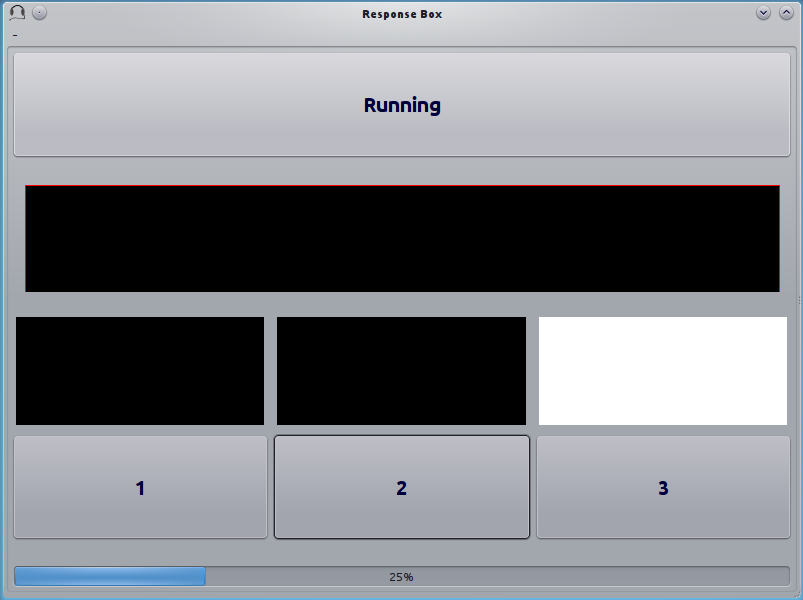
\includegraphics[scale=0.6]{Figures/response_box.png}
   \label{fig:response_box}
 \end{figure}

\begin{figure}[!h]
   \caption{The Control Window}
   \centering
   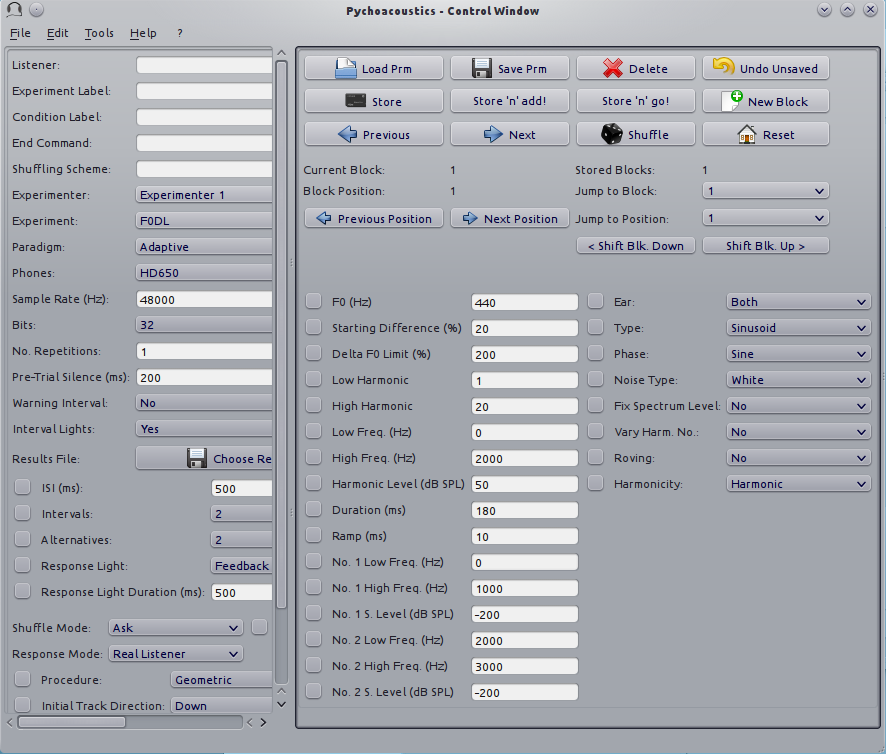
\includegraphics[scale=0.55]{Figures/control_window.png}
   \label{fig:control_window}
 \end{figure}

I started writing \texttt{pychoacoustics} for fun and for the sake of learning around 2008 while doing my PhD with Professor Chris Plack at Lancaster University. At that time we were using in the lab a MATLAB program called the ``Earlab'' written by Professor Plack. \texttt{pychoacoustics} has been greatly influenced and inspired by the ``Earlab'', and it reproposes many of the same features that the ``Earlab'' provides. For this reason, as well as for the patience he had to teach me audio programming I am greatly indebted to Professor Plack. %The ``Earlab'' has a venerable history, and was ported to various platforms and programming languages before reaching its MATLAB incarnation. \texttt{pychoacoustics} was initially written using the wxWidgets toolkit, and was 



%%% Local Variables: 
%%% mode: latex
%%% TeX-master: "pychoacoustics_manual"
%%% End: 


\chapter{Installation}

\texttt{pychoacoustics} has been successfully installed and used on Linux and Windows platforms, since it is entirely written in python it should be fully cross-platform and should work on the Mac as well, but this has never been tested. \texttt{pychoacoustics} depends on the installation of a handful of other programs:
\begin{itemize}
\item Python (version 3) \href{http://www.python.org/}{http://www.python.org/}
\item pyqt4 \href{http://www.riverbankcomputing.co.uk/software/pyqt/download}{http://www.riverbankcomputing.co.uk/software/pyqt/download}
\item numpy \href{http://sourceforge.net/projects/numpy/files/}{http://sourceforge.net/projects/numpy/files/}
\item scipy \href{http://sourceforge.net/projects/scipy/files/}{http://sourceforge.net/projects/scipy/files/}
\end{itemize}
these programs need to be installed manually. Once these programs are installed you can proceed with the installtion of \texttt{pychoacoustics}. %At this time there is no Linux package or Windows executable to automatically install \texttt{pychoacoustics}, however the installation is quite simple. %It can be installed either as a standard python program, using \verb+python setup.py install+ or it can simply unpacked 

\section{Installation on Linux} 
%On debian based platforms the dependencies can be installed using
%\begin{verbatim}
%sudo apt-get install python3 pyqt4 numpy scipy
%\end{verbatim}
Binary deb packages for recent debian-based distributions are provided (starting from Wheezy), and can be installed
using gdebi which automatically handles dependencies. For other linux systems,
once all of the dependencies have been installed,
\texttt{pychoacoustics} can be installed as a standard python package using
\begin{verbatim}
sudo python3 setup.py install
\end{verbatim}
you can then invoke \texttt{pychoacoustics} from a terminal by typing the command 
\begin{verbatim}
pychoacoustics.pyw
\end{verbatim}

\section{Installation on Windows}

\subsection{Using the binary installer}
After installing the dependencies (\texttt{python}, \texttt{pyqt4}, \texttt{numpy}, and \texttt{scipy}), simply double click on the \texttt{pychoacoustics}
windows installer to start the installation procedure. Currently the installer does not provide a launcher.
There is, however, a file called \texttt{pychoacoustics-qt4.bat} inside the source distribution of pychoacoustics that
after some modifications can be used as a launcher. The content of the file is the following:
\begin{verbatim}
C:\Python32\python "C:\Python32\site-packages\pychoacoustics.pyw" 
%1 %2 %3 %4 %5 %6 %7 %8
\end{verbatim}
The first statement \verb+C:\Python32\python+ is the path to the Python executable.
The second statement is the path to the main file of the \texttt{pychoacoustics} app.
You simply need to replace those two statements to reflect the Python installation on your system.

You can place the \texttt{.bat} launcher wherever you want, for example on your \texttt{Desktop}
folder. Simply double click on it, and \texttt{pychoacoustics} should start.
%The installer should create a launcher on the desktop, and a launcher on the start menu \footnote{Due to a bug, when you uninstall \texttt{pychoacoustics}, the launchers on the desktop and on the start menu may not be automatically removed. You can however remove them manually. For the launcher on the start manu, simply right click on it and select ``Remove''}.

\subsection{Installing from source}
After installing the dependencies, it is recommended to add the directory 
where the Python executable resides to the system \verb+PATH+. In this way 
you can call \texttt{python} from a \texttt{DOS} shell by simply typing its 
name, rather than typing the full path to the Python executable.

By default \texttt{python} is installed in \verb+C:+. The name of the Python
directory depends on its version number, for example, if you installed Python 
version 3.2, the python directory will be \verb+C:\Python32+. To add this 
directory to the system path go to \texttt{My Computer} and click \texttt{Properties}, 
then click \texttt{Advanced System Settings}. In the \texttt{System Properties} window 
click \texttt{Environment Variables}. There you will find an entry called \texttt{Path}. 
Select it and click \texttt{Edit}. Be careful not to remove any of the entries that are 
already written there because it could corrupt your system. Simply append the name of 
the full path of the folder where \texttt{python} is installed, at the end of the other entries.

To install \texttt{pychoacoustics} from source, unpack the \texttt{pychoacoustics} 
\texttt{.zip} file containing the source code. Open a \texttt{DOS} shell and \texttt{cd} 
to the directory where you unzipped pychoacoustics. The program can then be installed 
as a standard python package using the following command:
\begin{verbatim}
python setup.py install
\end{verbatim}
If you have installed the dependencies, you can also use pychoacoustics without installing it.
Open a \texttt{DOS} shell, \texttt{cd} to the directory where you unzipped pychoacoustics and launch it with the following command:
\begin{verbatim}
python pychoacoustics.pyw
\end{verbatim}
As mentioned in the previous section, there is also a \texttt{.bat} launcher that can be used to launch
\texttt{pychoacoustics} without needing to open a \texttt{DOS} shell each time. You can read the previous
section for further info.



%%% Local Variables: 
%%% mode: latex
%%% TeX-master: "pychoacoustics_manual"
%%% End: 

\chapter{Graphical User Interface}

The user interface is divided in two windows: the ``Control Window'' and the ``Response Box''. The ``Control Window'' 
is used to set the experimental parameters, while the ``Response Box'' 
is the interface that the listeners use to give their responses.

\section{Quickstart}
When \texttt{pychoacoustics} is launched, the ``Control Window'' displays the default parameters for 
the ``Audiogram'' experiment. You can select another experiment using the ``Experiment'' 
drop-down menu, and edit any of the parameter fields you want to modify. Once you're 
satisfied with the parameters, you can store them by pressing the ``Store'' button. 
This stores one experimental block with the chosen parameters. At this point you 
can either start running the experiment by pressing the ``Start'' button on the 
``Response Box'', or you can add more experimental blocks by clicking on the ``New Block'' button.

To save the parameters to a file click on the ``Save Prm'' button. 
Parameter files that have been saved in this way can be later loaded 
into the program by using the ``Load Prm'' button.

To save the results of your experiment to a file, click on the ``Save Results'' button. 
If you have forgotten to specify a results file in this way, \texttt{pychoacoustics} 
will save the results in a file called \texttt{test.txt} in the working directory. 

\section{The Control Window}
The control window contains a set of widgets to manage the setup of the experiments,
running the experiments, processing results files and managing application preferences. 
Some of the widgets are general, and some of them are specific either to a given
paradigm (e.g.\ adaptive vs constant stimuli paradigm) or to a given experiment.

In the next section the function of these widgets will be explained, starting with the
widgets that are general to all experiments and paradigms.

\subsection{General Widgets (left panel)}
\label{sec:gui_left_panel}
\begin{itemize}
\item \textbf{Listener} This is simply a label that you can use to identify
the person who is running the experiment. This label will be written in the 
header of the results file.
\item \textbf{Experiment Label}. This is a label to identify the experiment 
you are running. This label will be written in the 
header of the results file.
\item \textbf{Session} This is a label to identify the experimental session,
it can be a number or a string. This label will be written in the 
header of the results file.
\item \textbf{Condition Label} This is a label to identify the experimental
condition of the current block of trials. It is optional, but it may be useful when
sorting the experimental results.
\item \textbf{End Command} Here you can write an operating system command 
(e.g.\ a bash command on Unix systems or a DOS command on Windows systems) to 
be performed at the end of the experimental session. 
This could be used to run a custom script to analyse the result files,
make a backup of the results files or other purposes. There are some variables
that can be accessed with a special string, such as the name of the results
file. These are listed in Section~\ref{sec:end_cmd} Table~\ref{tab:end_cmd}. Please, refer to that section 
for further info on how to use them. 

\item \textbf{Shuffling Scheme} By default when you click the ``Shuffle'' button, \texttt{pychoacoustics} randomly shuffles all blocks, here you can specify
different shuffling schemes (e.g.\ shuffle the first four blocks among themselves and the last four blocks among themselves).
Please refer to Section~\ref{sec:shuffling} for more details.

\item \textbf{Results File} Select a file for saving the results. Selecting an existing file will never
overwrite its content, it will simply append the new results to its content. If no file is selected,
the results will be saved in a file called \texttt{test.txt} in the current working directory. You can select
a file to save the results even after you have started a block of trials, the results get written to
the file only at the end of the block.

\item \textbf{Experimenter} Here you can select one of the experimenters listed in the
experimenter database. Please refer to Section~\ref{sec:experimenters_dialog} for further info on the experimenter
database and how it can be used. 
\item \textbf{Experiment} Selects the experiment for the current block.
\item \textbf{Paradigm} Selects the paradigm (e.g. adaptive, constant, etc\ldots) 
for the current block. The list of paradigms available depends on the experiment
that is selected. 
\item \textbf{Phones} Choose from one of the phone models stored in the phones database.
Please, refer to Section~\ref{sec:phones_dialog} for further info on how to enter phones and calibration values
in the database.
\item \textbf{Sample Rate (Hz)} Set the sampling rate of the sounds to be played. Any value
can be entered in the text fields. However, you should enter a value that is supported 
by your soundcard. A value that is not supported by your souncard may lead to issues,
although it's more likely that your soundcard will perform an automatic sample rate
conversion.
\item \textbf{Bits} Set the bit depth that \texttt{pychoacoustics} uses to store sounds 
to a wav file or play them. Currently values of 16 and 32 bits are supported. 
A value of 32 bits can be used for 24-bit soundcards. Notice that to achieve 24-bit output 
requires both a 24-bit souncard and a play command that can output 24-bit sounds. Therefore 
selecting a value of 32 bits here does not guarantee 24-bit playback even if you have a 24-bit souncard. 
Please, refere to Section~\ref{sec:sound_output} for further information on this issue.

\item \textbf{Repetitions} Set the number of times the sequence of blocks stored in memory should be repeated. If the ``Shuffle Mode'' (see below) is 
set to ``auto'', each time a new repetition starts the block positions will be shuffled. If the ``Shuffle Mode'' is set to ``Ask'', each time a new
repetition starts the user will be asked if s/he wants to shuffle the block positions. The ``Reset'' button resets the number of repetitions to zero.

\item \textbf{Pre-Trial Silence (ms)} Set a silent time interval before the start of each trial. 

\item \textbf{Warning Interval} Choose whether to present a warning light at the beginning of each trial. 

\item \textbf{Warning Interval Duration (ms)} Sets the duration of the warning interval light.
  This widget is shown only if the warning interval chooser is set to ``Yes''.

\item \textbf{Warning Interval ISI (ms)} Sets the duration of the silent interval between the end of warning interval and the start of the first observation interval.
  This widget is shown only if the warning interval chooser is set to ``Yes''.

\item \textbf{Pre-Trial Interval} Choose whether to present a pre-trial interval. This widget is shown only for experiments that have a pre-trial interval option.

\item \textbf{Pre-Trial Interval ISI (ms)} Sets the duration of the silent interval between the end of pre-trial interval and the start of the first observation interval.
  This widget is shown only if the current experiment has a pre-trial interval option and the pre-trial interval chooser is set to ``Yes''.

\item \textbf{Response Light} Set the type of response light at the end of each trial. "Feedback" will
flash a green (correct response) or red (incorrect response) light. "Neutral" will flash a white light.
"None" will not flash any light (there will nonetheless be a silent interval equal to the response light duration, see below).

\item \textbf{Response Light Duration (ms)} Set the duration of the response light.
 
\item \textbf{Shuffle Mode} If the ``Shuffle Mode'' is ``auto'', the  block presentation positions 
will be automatically shuffled at the beginning of a series of blocks. If the ``Shuffle Mode'' 
is ``Ask'', at the beginning of a series of blocks the user will be asked if the block presentation
positions should be shuffled or not. If the ``Shuffle Mode'' is ``No'', the block presentation positions
will not be automatically shuffled at the beginning of a series of blocks. 
See Section~\ref{sec:shuffling} for further information on shuffling the block presentation positions.

\item \textbf{Response Mode} When ``Real Listener'' is selected, \texttt{pychoacoustics} waits for responses
from a human listener. When ``Automatic'' is selected the program will give responses by itself with a certain
percentage correct, that can be specified in the ``Percent Correct (\%)'' text field. This mode is mostly
useful for debugging purposes, however it can also be used for experiments in which the
participants are passively listening to the stimuli (e.g. some neuroimaging experiments that record cerebral responses
rather than behavioural responses). In ``Simulated Listener'' mode \texttt{pychoacoustics} will give responses
on the bases of an auditory model. This model needs to be specified in the experiment file, the ``Simulated Listener'' mode
provides just a hook to redirect the control flow to your model.
Please, refer to Section~\label{sec:response_mode} for more information.


\end{itemize}

\subsection{General Widgets (right panel)}
\begin{itemize}
\item \textbf{Load Prm} Load in memory experimental parameters stored in a \texttt{.prm} file. See section~\ref{sec:parameters_files} for more info.
\item \textbf{Save Prm} Save experimental parameters stored in memory in a \texttt{.prm} file. See section~\ref{sec:parameters_files} for more info.
\item \textbf{Delete} Delete the current block from the blocks list.
\item \textbf{Undo Unsaved} Reset the parameters in the current block to the parameters that were last saved.
\item \textbf{Store} Store the parameters changes in memory.
\item \textbf{Store 'n' add} Store the parameter changes in memory and add a new parameters block.
\item \textbf{Store 'n' go} Store the parameter changes in memory and move to the next block storage point.
\item \textbf{New Block} Create a new parameters block (the parameters of the current block will be copied in the new one).
\item \textbf{Previous} Move to the previous block storage point.
\item \textbf{Next} Move to the next block storage point.
\item \textbf{Shuffle} Shuffle the block presentation positions.
\item \textbf{Reset} Reset the block presentation positions and move to the first block position.
\item \textbf{Jump to Block} Jump to a given block storage point.
\item \textbf{Previous Position} Move to the previous block presentation position.
\item \textbf{Next Position} Move to the next block presentation position.
\item \textbf{Jump to Position} Jump to the given block presentation position.
\item \textbf{Shift Blk. Down} Shift the current block to a lower storage point.
\item \textbf{Shift Blk. Up} Shift the current block to a higher storage point.
\end{itemize}

\subsection{Paradigm Widgets}
\subsubsection{Adaptive Paradigm Widgets}

\begin{itemize}
\item \textbf{Procedure} If ``Arithmetic'' the quantity defined by the step size will be added or subtracted to the parameter that is adaptively changing. 
  If ``Geometric'' the parameter that is adaptively changing will be multiplied or divided by the quantity defined by the step size.
\item \textbf{Initial Track Direction} This determines when the first turpoint will be called. If the initial track direction is ``Down'' the first turnpoint will be called
  the first time the adaptive track turns upward. If the initial track direction is ``Up'' the first turnpoint will be called
  the first time the adaptive track turns downward.
\item \textbf{Rule Down} Set the number of consecutive correct responses needed to subtract the current step size from the adaptive parameter (for arithmetic procedures) or divide
  the adaptive parameter by the current step size (for geometric procedures).
\item \textbf{Rule Up} Set the number of consecutive incorrect responses needed to add the current step size to the adaptive parameter (for arithmetic procedures) 
  or multiply the adaptive parameter by the current step size (for geometric procedures).
\item \textbf{Initial Turnpoints} Set the number of initial turnpoints. The initial turnpoints serve to bring quickly the adaptive track towards the listener's threshold.
  These turnpoints are not included in the threshold estimate. 
\item \textbf{Total Turnpoints} Set the number of total turnpoints. The number of total turnpoints is equal to the number of initial turnpoints that are not included in the threshold estimate
  plus the number of turnpoints that you want to use for the threshold estimate.
\item \textbf{Step Size 1} Set the step size for the initial turnpoints.
\item \textbf{Step Size 2} Set the step size to be used after the number of initial turnpoints has been reached.
\end{itemize}


\subsubsection{Weighted Up/Down Paradigm Widgets}

\begin{itemize}
\item \textbf{Procedure} If ``Arithmetic'' the quantity defined by the step size will be added or subtracted to the parameter that is adaptively changing. 
  If ``Geometric'' the parameter that is adaptively changing will be multiplied or divided by the quantity defined by the step size.
\item \textbf{Initial Track Direction} This determines when the first turpoint will be called. If the initial track direction is ``Down'' the first turnpoint will be called
  the first time the adaptive track turns upward. If the initial track direction is ``Up'' the first turnpoint will be called
  the first time the adaptive track turns downward.
\item \textbf{Percent Correct Tracked} Set the percentage correct point on the psychometric function to be tracked by the adaptive procedure. The ratio of the ``Up'' and ``Down'' steps
  is automatically adjusted by the software to satisfy this criterion.
\item \textbf{Initial Turnpoints} Set the number of initial turnpoints. The initial turnpoints serve to bring quickly the adaptive track towards the listener's threshold.
  These turnpoints are not included in the threshold estimate. 
\item \textbf{Total Turnpoints} Set the number of total turnpoints. The number of total turnpoints is equal to the number of initial turnpoints that are not included in the threshold estimate
  plus the number of turnpoints that you want to use for the threshold estimate.
\item \textbf{Step Size 1} Set the ``Down'' step size for the initial turnpoints. The ``Up'' step size is automatically calculated to satisfy the ``Percent Correct Tracked'' criterion.
\item \textbf{Step Size 2} Set the ``Down'' step size to be used after the number of initial turnpoints has been reached. The ``Up'' step size is automatically calculated to satisfy the ``Percent Correct Tracked'' criterion.
\end{itemize}
\subsubsection{Adaptive Interleaved Paradigm Widgets}

\begin{itemize}
\item \textbf{Procedure} If ``Arithmetic'' the quantity defined by the step size will be added or subtracted to the parameter that is adaptively changing. 
  If ``Geometric'' the parameter that is adaptively changing will be multiplied or divided by the quantity defined by the step size.
\item \textbf{No. Tracks} Set the number of adaptive tracks.
\item \textbf{Max. Consecutive Trials x Track} Set the maximum number of consecutive trials per track. 
\item \textbf{Turnpoints to Average} Since track selection is pseudo-random, it may happen that for a track the number of total turnpoints collected is greater
  than the number of total turnpoints requested for that track. If ``All final step size (even)'' is selected, the threshold will be estimated using all
  the turnpoints collected after the initial turnpoints, unless the number of these turnpoints is odd, in which case the first of these turnpoints will be discarded.
  If ``First N final step size'' is selected the threshold will be estimated using only the number of requested turnpoints collected after the initial turnpoints.
  If ``Last N final step size'' is selected the threshold will be estimated using only the last $N$ turnpoints, where $N$ equals the number of requested turnpoints.
\item \textbf{Initial Track X Direction} This determines when the first turpoint will be called for track number $X$. If the initial track direction is ``Down'' the first turnpoint will be called
  the first time the adaptive track turns upward. If the initial track direction is ``Up'' the first turnpoint will be called
  the first time the adaptive track turns downward.
\item \textbf{Rule Down Track X} Set the number of consecutive correct responses needed to subtract the current step size from the adaptive parameter (for arithmetic procedures) or divide
  the adaptive parameter by the current step size (for geometric procedures) for track number $X$.
\item \textbf{Rule Up Track X} Set the number of consecutive incorrect responses needed to add the current step size to the adaptive parameter (for arithmetic procedures) 
  or multiply the adaptive parameter by the current step size (for geometric procedures) for track number $X$.
\item \textbf{Initial Turnpoints Track X} Set the number of initial turnpoints for track number $X$. The initial turnpoints serve to bring quickly the adaptive track towards the listener's threshold.
  These turnpoints are not included in the threshold estimate. 
\item \textbf{Total Turnpoints Track X} Set the number of total turnpoints for track number $X$. The number of total turnpoints is equal to the number of initial turnpoints that are not included in the threshold estimate
  plus the number of turnpoints that you want to use for the threshold estimate.
\item \textbf{Step Size 1 Track X} Set the step size for the initial turnpoints for track number $X$.
\item \textbf{Step Size 2 Track X} Set the step size to be used after the number of initial turnpoints has been reached for track number $X$.
\end{itemize}

\subsubsection{Weighted Up/Down Interleaved Paradigm Widgets}

\begin{itemize}
\item \textbf{Procedure} If ``Arithmetic'' the quantity defined by the step size will be added or subtracted to the parameter that is adaptively changing. 
  If ``Geometric'' the parameter that is adaptively changing will be multiplied or divided by the quantity defined by the step size.
\item \textbf{No. Tracks} Set the number of adaptive tracks.
\item \textbf{Max. Consecutive Trials x Track} Set the maximum number of consecutive trials per track. 
\item \textbf{Turnpoints to Average} Since track selection is pseudo-random, it may happen that for a track the number of total turnpoints collected is greater
  than the number of total turnpoints requested for that track. If ``All final step size (even)'' is selected, the threshold will be estimated using all
  the turnpoints collected after the initial turnpoints, unless the number of these turnpoints is odd, in which case the first of these turnpoints will be discarded.
  If ``First N final step size'' is selected the threshold will be estimated using only the number of requested turnpoints collected after the initial turnpoints.
  If ``Last N final step size'' is selected the threshold will be estimated using only the last $N$ turnpoints, where $N$ equals the number of requested turnpoints.
\item \textbf{Initial Track X Direction} This determines when the first turpoint will be called for track number $X$. If the initial track direction is ``Down'' the first turnpoint will be called
  the first time the adaptive track turns upward. If the initial track direction is ``Up'' the first turnpoint will be called
  the first time the adaptive track turns downward.
\item \textbf{Percent Correct Tracked} Set the percentage correct point on the psychometric function to be tracked by the adaptive procedure for track number $X$. The ratio of the ``Up'' and ``Down'' steps
  is automatically adjusted by the software to satisfy this criterion.
\item \textbf{Initial Turnpoints Track X} Set the number of initial turnpoints for track number $X$. The initial turnpoints serve to bring quickly the adaptive track towards the listener's threshold.
  These turnpoints are not included in the threshold estimate. 
\item \textbf{Total Turnpoints Track X} Set the number of total turnpoints for track number $X$. The number of total turnpoints is equal to the number of initial turnpoints that are not included in the threshold estimate
  plus the number of turnpoints that you want to use for the threshold estimate.
\item \textbf{Step Size 1 Track X} Set the ``Down'' step size for the initial turnpoints for track number $X$. The ``Up'' step size is automatically calculated to satisfy the ``Percent Correct Tracked'' criterion.
\item \textbf{Step Size 2 Track X} Set the ``Down'' step size to be used after the number of initial turnpoints has been reached for track number $X$. The ``Up'' step size is automatically calculated to satisfy the ``Percent Correct Tracked'' criterion.
\end{itemize}


\subsubsection{Constant m-Intervals n-Alternatives Paradigm Widgets}

\begin{itemize}
\item \textbf{No. Trials} Set the number of trials to be presented in the current block.
\item \textbf{No. Practice Trials} Set the number of practice trials to be presented in the current block. Practice trials are presented at the
  beginning of the block; the responses to these trials are not included in the statistics.
\end{itemize}

\subsubsection{Multiple Constants m-Intervals n-Alternatives Paradigm Widgets}

\begin{itemize}
\item \textbf{No. Trials} Set the number of trials to be presented in the current block for each condition.
\item \textbf{No. Practice Trials} Set the number of practice trials to be presented in the current block for each condition. The responses to these trials are not included in the statistics.
\item \textbf{No. Differences} Set the number of conditions to be used in the current block.
\end{itemize}

\subsubsection{Constant 1-Interval 2-Alternatives Paradigm Widgets}

\begin{itemize}
\item \textbf{No. Trials} Set the number of trials to be presented in the current block.
\item \textbf{No. Practice Trials} Set the number of practice trials to be presented in the current block. Practice trials are presented at the
  beginning of the block; the responses to these trials are not included in the statistics.
\end{itemize}

\subsubsection{Multiple Constants 1-Interval 2-Alternatives Paradigm Widgets}

\begin{itemize}
\item \textbf{No. Trials} Set the number of trials to be presented in the current block for each condition.
\item \textbf{No. Practice Trials} Set the number of practice trials to be presented in the current block for each condition. The responses to these trials are not included in the statistics.
\item \textbf{No. Differences} Set the number of conditions to be used in the current block.
\end{itemize}

\subsubsection{1-Pair Same/Different Paradigm Widgets}

\begin{itemize}
\item \textbf{No. Trials} Set the number of trials to be presented in the current block.
\item \textbf{No. Practice Trials} Set the number of practice trials to be presented in the current block. Practice trials are presented at the
  beginning of the block; the responses to these trials are not included in the statistics.
\end{itemize}

\subsection{The Menu Bar}
A screenshot of the menu bar is shown in Figure~\ref{fig:menuBar}. This bar is located in the upper left corner of the ``Control Window''. Each menu will be described below.
\begin{figure}[!h]
   \caption{The menu bar.}
   \centering
   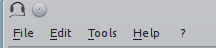
\includegraphics{Figures/menuBar.png}
   \label{fig:menuBar}
 \end{figure}

\subsubsection{The File Menu}
\begin{itemize}
\item \textbf{Process Results} Process block summary results files to obtain 
session summary results files. For more info see Section~\ref{sec:proc_res_dia}.
\item \textbf{Process Results Table} Process block summary results table files to obtain 
session summary table results files. For more info see Section~\ref{sec:proc_res_dia}.
\item \textbf{Open Results File} Open the file where \texttt{pychoacoustics} is currently saving data with the default text editor.
\item \textbf{Exit.} Close \texttt{pychoacoustics}.

\end{itemize}

\subsubsection{The Edit Menu}
\begin{itemize}
\item \textbf{Edit Preferences} Edit application preferences. See Section~\ref{sec:pref_dialog} for further info.
\item \textbf{Edit Phones} Edit the phones database, and set the calibration levels for your phones. See Section~\ref{sec:phones_dialog} for further info.
\item \textbf{Edit Experimenters} Edit the experimenters database. See Section~\ref{sec:experimenters_dialog} for further info.
\end{itemize}

\subsubsection{The Tools Menu}
\begin{itemize}
\item \textbf{Swap Blocks} Swap the storage position of two parameter blocks.
\end{itemize}

\subsubsection{The Help Menu}
\begin{itemize}
\item \textbf{Fortunes} Show psychoacoustics fortunes. I'm always collecting new ones, so if you happen to know any interesting ones, please, e-mail them to me so that I can add them to the collection.
\item \textbf{About pychoacoustics} Show information about the licence, the version of the software and the version of the libraries it depends on.
\end{itemize}

\subsubsection{The ``what's this?'' Button.}
If you click on this button, and then click on a widget,
you can get some information about the widget (this is not implemented
for all widgets).

\section{Process Results Dialog}
\label{sec:proc_res_dia}
Figure~\ref{fig:proc_res_dia} show a screenshot of the process results dialog. The dialog is the same for all
procedures, except that for procedures in which \emph{d'} is computed, there is an additional checkbox asking whether to
apply a correction to hit/false alarm rates of zero or one. For information on the format of the result files,
please see Section~\ref{sec:results_files}. 
\begin{figure}[!h]
   \caption{The process results dialog.}
   \centering
   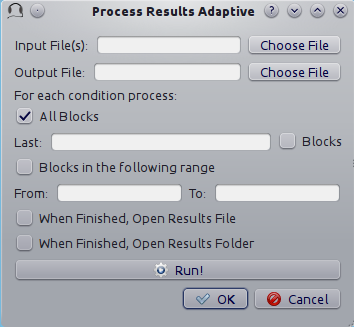
\includegraphics{Figures/proc_res_dia.png}
   \label{fig:proc_res_dia}
 \end{figure}
\begin{itemize}
\item \textbf{Input File(s)} Give the filepath of one or more files to be processed. The ``Choose File'' button can be used to select the file(s). Multiple filepaths
  should be separated by a semicolon ``\texttt{;}''.
\item \textbf{Output File} Give the filename of the output file.
\item \textbf{For each condition process:}
  \begin{itemize}
  \item \textbf{All Blocks} If checked, all blocks in the result file(s) will be processd.
  \item \textbf{Last X Blocks} If checked, only the last $X$ blocks will be processed.
  \item \textbf{Blocks in the following range} If checked, only blocks in the specified range will be processed (indexing starts from 1).
  \end{itemize}
\item \textbf{d-prime correction} If checked, convert hit rates of $0$ and $1$ to $1/2N$ and $1-1/(2N)$ respectively, where $N$ is the number of trials, to avoid infinite values of \emph{d'} \cite<see>[p.\ 8]{Macmillan2005}.
  This checkbox is available only for some paradigms.
\item \textbf{When finished, open results file} If checked, the output file will be opened in the default text editor when processing has finished.
\item \textbf{When finished, open results folder} If checked, the folder containing the output file will be opened when processing has finished.
\item \textbf{Run!} Click this button to process the result files.
 
\end{itemize}


\section{Edit Preferences Dialog}
\label{sec:pref_dialog}
The preferences dialog is divided into several tabs. These are described in turn below.

\subsection{General}
\label{sec:pref_dialog_gen}
\begin{itemize}
\item \textbf{Language (requires restart)} Choose the application language. At the moment and for the foreseeable future
  only English is supported.
\item \textbf{Country (requires restart)} Set the country locale to be used for the application. Some things (e.g.\ the way dates are written in result files depend on this setting.
\item \textbf{Response Box Language (requires restart)} Choose the language to be used for the ``Response Box''. This set the language to be used for the button labels and other
  GUI elements that the experimental listener is presented with. 
\item \textbf{Response Box Country (requires restart)} Set the country locale for the response box.
\item \textbf{csv separator} Choose the separator field to be used  when writing the csv tabular result files.
\item \textbf{Warn if listener name missing} If checked, pop up a warning message if the listener name is missing at the beginning of a session.
\item \textbf{Warning if session label missing} If checked, pop up a warning message if the session label is missing at the beginning of a session.
\item \textbf{Process results when finished} If checked, process automatically the block summary file to generate the session summary file at the end of the experiment.
\item \textbf{d-prime correction} If checked, when automatically processing result files, convert hit rates of $0$ and $1$ to $1/2N$ and $1-1/(2N)$ respectively, where $N$ is the number of trials, to avoid infinite values of \emph{d'} \cite<see>[p.\ 8]{Macmillan2005}.
\item \textbf{Max Recursion Depth (requires restart)} Set the maximum recursion depth of the Python interpreter stack. This setting should be changed only if you intend
  to run \texttt{pychoacoustics} in automatic or simulated listener response mode. Beware, setting a max recursion depth value smaller than the default value may cause
  \texttt{pychoacoustics} to crash or not even start. In case \texttt{pychoacoustics} does not start because of this, delete your preferences settings file to restore
  the default max recursion depth value.
 
\end{itemize}

\subsection{Sound}
\label{sec:pref_dialog_sound}
\begin{itemize}
\item \textbf{Play Command} Set an internal or external command to play sounds.
\item \textbf{Device} Set the soundcard to be used to play sounds. This chooser is available
  only for certain internal play commands (currently alsaaudio and pyaudio).
\item \textbf{Buffer Size (samples)} Set the buffer size in number of samples to be used to output sounds. This chooser is available only for certain internal play commands (currently alsaaudio and pyaudio).
\item \textbf{Default Sampling Rate} Set the default sampling rate.
\item \textbf{Default Bits} Set the default bit depth.
\item \textbf{Wav manager (requires restart)} Choose the wav manager.
\item \textbf{Write wav file} Write wav files with the sounds played on each trial in the current \texttt{pychoacoustics} working directory.
\item \textbf{Write sound sequence segment wavs} For sound sequences, write a wav file for each segment of the sequence in the current \texttt{pychoacoustics} working directory.
\item \textbf{Append silence to each sound (ms)} Append a silence of the given duration at the end of each sound. This is useful on some versions of the Windows operating system that may cut the sound buffer before it has ended resulting in audible clicks.
\end{itemize}

\subsection{Notifications}
\label{sec:pref_dialog_notify}
\begin{itemize}
\item \textbf{Play End Message} If checked, play a wav file at the end of the experiment.
  This could be short message to let the listeners know they have finished and thank them
  for their participation in the experiment. One or more wav files need to be set through
  the ``Choose wav'' button for this work.
\item \textbf{Choose wav} Choose the wav file to be played as the end message. Clicking on this button 
  brings up another dialog where you can select the wav files to be played and their output RMS.
  Only one of the wav files listed here and with the ``Use'' flag set to \ding{51} will be randomly chosen
  and played.
\item \textbf{blocks before end of experiment} Set how many blocks before the end of the experiment
  the two actions listed below (send notification e-mail and execute custom command) should be performed.
\item \textbf{Send notification e-mail} If checked, send a notification e-mail to the experimenter
  to notify her that the experiment is about to finish.
\item \textbf{Execute custom command} If checked, execute an operating system command before the end
  of the experiment. This command could be used to automatically send an sms for example.
\item \textbf{Send data via e-mail} At the end of the experiment, send the results file to the experimenter .
\item \textbf{Execute custom command} At the end of the experiment, execute an operating system command.
\item \textbf{Outgoing Server (SMTP)} Set the name of the SMTP server to be used by \texttt{pychoacoustics} to send e-mails.
\item \textbf{Port} Set the port number for the SMTP server.
\item \textbf{Security} Set the security protocol for network exchanges with the SMTP server.
\item \textbf{Server requires identification} Check this if the SMTP server requires identification.
\item \textbf{Username} Set the username for the SMTP server.
\item \textbf{Password} Set the password for the SMTP server.
\item \textbf{Send test e-mail} Send a test e-mail to check that the server settings are OK.
\end{itemize}

\subsection{EEG}
\label{sec:pref_dialog_eeg}
\begin{itemize}
\item \textbf{ON Trigger} The ON trigger value (decimal).
\item \textbf{OFF Trigger} The OFF trigger value (decimal).
\item \textbf{Trigger Duration (ms)} The duration of the trigger in milliseconds.
\end{itemize}


\section{Edit Phones Dialog}
\label{sec:phones_dialog}
A screenshot of the ``Edit Phones'' dialog is shown in Figure~\ref{fig:phones_dialog}.
\begin{figure}[!hbt]
   \caption{The edit phones dialog.}
   \centering
   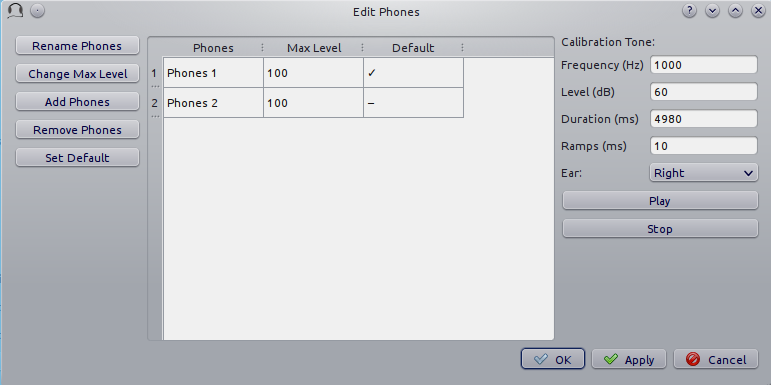
\includegraphics[scale=.65]{Figures/phones_database.png}
   \label{fig:phones_dialog}
 \end{figure}
Most of the fields should be pretty much self-explanatory. Using this dialog you can add headphones/earphones
models to the phones database. The phone with the ``Default'' flag set to \ding{52} will be selected by default when \texttt{pychoacoustics} is started. In the ``Max Level'' field you should enter the level in dB SPL that is output by the phone for a full amplitude sinusoid. This value will be used by \texttt{pychoacoustics} to output sounds at specific levels in dB SPL. On the rightmost panel of the dialog you have facilities to play a sinusoid with a specified level. You can use these facilities to check with a SPL meter (or a voltmeter depending on how you're doing it) that the actual output level corresponds to the desired output level. Using these facilities you can also play a full amplitude sinusoid: you need to set the level of the sinuoid to the ``Max Level'' of the phone (whatever it is). Be careful because it can be very loud!

\section{Edit Experimenters Dialog}
\label{sec:experimenters_dialog}
A screenshot of the ``Edit Experimenters'' dialog is shown in Figure~\ref{fig:experimenters_dialog}.
\begin{figure}[!h]
   \caption{The edit experimenters dialog.}
   \centering
   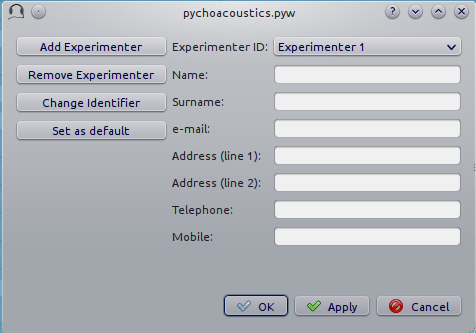
\includegraphics{Figures/experimenter_database.png}
   \label{fig:experimenters_dialog}
 \end{figure}
Most of the fields should be pretty much self-explanatory. Here you can add
the details of the experimenters that work in your lab in the experimenter
database. The main functions of this database at the moment are a) writing
the experimenter name in the results file; b) using the experimenter e-mail 
for sending notifications and/or results files (see Section~\ref{sec:pref_dialog_notify}).



\section{The Response Box}

The ``response box'' consists of a large button (the ``status button'') that is used to start a block of trials, a feedback light to display trial by trial feedback, interval lights to mark observation intervals, and response buttons. The responses can be given either by means of mouse clicks, or using the numeric keypad (key ``1'' for the first button, key ``2'' for the second button etc\ldots). Responses given before all observation intervals have been presented are not accepted. 

The status button can be activated  by pressing the \texttt{Ctrl+R} shortcut.  At the start of each block the label of the ``Status Button'' is set to ``Start''. Once the listener starts a block of trials the label of the status button changes to ``Running''. When a whole series of blocks is finished the label of the status button changes to ``Finish''. If no blocks are stored in memory the label of the status button is set to ``Wait''.

On the top left corner of the response box there is a semi-hidden menu signalled by a little hyphen (``-''). If you click on it you have access to two functions. The ``Show/Hide Control Window'' function can be used to hide the control window while the experiment is running. This is useful because it prevents the listener from accidentally changing your experimental parameters or accidentally closing \texttt{pychoacoustics} (the response box itself has no ``close'' button, so it is not possible to close that). The ``Show/Hide progress Bar'' function can be used to display a progress bar at the bottom of the response box. The progress bar estimates what percentage of the experiment has been completed. This estimate depends on the procedure used (for constant procedures it is based on the number of trials done, while for adaptive procedures it is based on the number of turnpoints reached) and on the specific parameters of a given experiment (trial duration, number of trials, or number or turnpoints, all of which can differ between blocks), so in some cases the estimate can be off the mark. The ``Show/Hide block progress Bar'' can be used to show the position of the current block and the total number of blocks. 





%%% Local Variables: 
%%% mode: latex
%%% TeX-master: "pychoacoustics_manual"
%%% End: 



\chapter{Command Line User Interface}
In order to automate certain tasks, or perform some advanced operations, \texttt{pychoacoustics} can be called from the command line with certain command line options. The following is the list of possible command line options:
\begin{itemize}
\item \verb+-h, --help+ Show help message.
\item \verb+-f, --file FILE+ Load parameters file \texttt{FILE}.
\item \verb+-r, --results FILE+  Save the results to file \texttt{FILE}.
\item \verb+-l, --listener LISTENER+ Set listener label to \texttt{LISTENER}.
\item \verb+-s, --session SESSION+ Set session label to \texttt{SESSION}.
\item \verb+-k, --reset+ Reset block positions.
\item \verb+-q, --quit+ Quit after finished.
\item \verb+-c, --conceal+ Hide Control and Parameters Windows.
\item \verb+-p, --progbar+ Show the progress bar.
\item \verb+-b, --blockprogbar+ Show the progress bar.
\item \verb+-a, --autostart+ Automatically start the first stored block.
\item \verb+-x, --recursion-depth+ Set the maximum recursion depth (this overrides the maximum recursion depth set in the preferences window).
\item \verb+-g, --graphicssystem+ sets the backend to be used for on-screen widgets and QPixmaps. Available options are raster and opengl.
\item \verb+-d, --display+ This option is only valid for X11 and sets the X display (default is \$DISPLAY).
\end{itemize}
each command line option has a short (single dash, one letter) and long (double dash, one word) form, for example to show the help message, you can use either of the two following commands:
\begin{verbatim}
$ pychoacoustics -h
$ pychoacoustics --help
\end{verbatim}


%%% Local Variables: 
%%% mode: latex
%%% TeX-master: "pychoacoustics_manual"
%%% End: 

\chapter{Psychophysics}
\section{Available Paradigms}
\label{sec:paradigms}
\subsubsection{Adaptive}
This paradigm implements the ``up/down'' adaptive procedures described by \citeA{Levitt1971}. It can be used with $n$-intervals, $n$-alternatives forced choice tasks, in which $n-1$ ``standard'' stimuli and a single ``comparison'' stimulus are presented each in a different temporal interval. The order of the temporal intervals is randomized from trial to trial. The ``comparison'' stimulus usually differs from the ``standard'' stimuli for a single characteristic (e.g.\ pitch or loudness), and the listener has to tell in which temporal interval it was presented. A classical example is the 2-intervals 2-alternatives forced choice task. Tasks that present a reference stimulus in the first interval, and therefore have $n$ intervals and $n-1$ alternatives are also supported \cite<see>[for an example of such tasks]{Grimault2002}.

\subsubsection{Adaptive Interleaved}
This paradigm implements the interleaved adaptive procedure described by \citeA{Jesteadt1980}.

\subsubsection{Weighted Up/Down}
This paradigm implements the weighted up/down adaptive procedure described by \citeA{Kaernbach1991}.

\subsubsection{Weighted Up/Down Interleaved}
This paradigm combines the interleaved adaptive procedure described by \citeA{Jesteadt1980} with the weighted up/down method described by \citeA{Kaernbach1991}.

\subsubsection{Constant m-Intervals n-Alternatives}
This paradigm implements a constant difference method for forced choice tasks with $m$-intervals and $n$-alternatives. For example, it can be used for running a 2-intervals, 2-alternatives forced choice frequency-discrimination task with a constant difference between the stimuli in the standard and comparison intervals.

\subsubsection{Constant 1-Interval 2-Alternatives}
This paradigm implements a constant difference method for tasks with a single observation interval and two response alternatives, such as the ``Yes/No'' signal detection task. 

\subsubsection{Constant 1-Pair Same/Different}
This paradigm implements a constant difference method for ``same/different'' tasks with a single pair of stimuli to compare.

\section{Available Experiments}





%%% Local Variables: 
%%% mode: latex
%%% TeX-master: "pychoacoustics_manual"
%%% End: 


\chapter{The \texttt{pychoacoustics} Engine}


\section{Sound Output}
\label{sec:sound_output}

\subsubsection{Sound Output on Linux}
On Linux systems \texttt{pychoacoustics} can either output sound (numpy arrays) directly to the soundcard, or
write a wav file for each sound and call an external command to play it. Currently, support for sending
sounds directly to the soundcard is possible only through the 
\href{http://pyalsaaudio.sourceforge.net/}{alsaaudio} python module.
This module is optional, and you need to install it yourself to be able to use it.

Once it is installed, it will be detected automatically and you will be able to 
select it as the ``Play Command'' in the sound preferences dialog. When you select
"alsaaudio" as the play command, if you have multiple soundcards, you can select the 
device to which the sound will be sent. There will be also an option to set the size
of the buffer that alsaaudio uses to play sounds. If the buffer is not filled completely
by a sound (buffer size greater than number of samples in the sound), it will be zero
padded. This may lead to some latency between the offset of a sound and the onset of the
following one. If you set a value smaller than one the buffer size will be automatically 
set to the number of samples in the sound that is being played.


Using an external command to play sounds generally works very well and is fast on modern hardware.
\texttt{pychoacoustics} tries to detect available play commands on your system each time it starts up.
On Linux systems, the recommended play command is \texttt{aplay}, which is installed by default on most Linux
distributions. \texttt{aplay} supports 24-bit output on 24-bit soundcards with appropriate Linux drivers.
Other possible play commands are \texttt{play}, which is provided by \href{http://sox.sourceforge.net/}{sox} and \texttt{sndfile-play}, which
is provided by the \href{http://www.mega-nerd.com/libsndfile/}{libsndfile} tools. You can call another program by choosing ``custom'' in the
``Play Command'' drop-down menu and spelling out the name of the command in the box below.

\subsubsection{Sound Output on Windows}
Currently, on Windows systems \texttt{pychoacoustics} cannot output sounds directly to the soundcard.
It writes instead a wav file and calls an external play commands to output the sound. The recommended 
play command is \texttt{winsound}. This command supports only 16-bit
output. 

Other possible play commands are \texttt{play}, which is provided by \href{http://sox.sourceforge.net/}{sox} 
and \texttt{sndfile-play}, which is provided by the \href{http://www.mega-nerd.com/libsndfile/}{libsndfile} tools. These programs need 
to be installed by the user. If they are in the system path, \texttt{pychoacoustics} will detect them automatically. 
I am not aware of any freely available play command that can output 24-bit sound in Windows. 
Portaudio could be a used, and the Python bindings provided by pyaudio have been recently ported to Python 3. 
I have not tried this solution (and don't have much time to do it), if you want to try it, you need to be aware that in order to get 24-bit audio, 
portaudio should be probably compiled with ASIO support, and compiling portaudio on Windows with ASIO support is quite a complicated process.
Note that external media players with a graphical user interface (like foobar2000) may not work well
with \texttt{pychoacoustics}. 


\section{Parameters Files}
\label{sec:parameters_files}
Parameters files are plain text files, that can be modified through \texttt{pychoacoustics} or through a text editor. They contain a header with information that applies to all all the experimental blocks stored in a parameters file, and sections corresponding to the parameters that are specific to each experimental block store in a parameters file.
The header contains the following fields:
\begin{itemize}
\item Phones
\item Shuffle Mode
\item Sample Rate
\item Bits
\item Experiment Label
\item End Command
\end{itemize}
You can refer to Section~\ref{sec:gui_left_panel} to know what each of these fields represents.

The sections that contain the parameters for each experimental block are subdivided into fields that are separated by one or more dots. You should not change this formatting when modifying parameters files.

A fragment from a parameters file is shown below:
\begin{verbatim}
Paradigm: Adaptive
Intervals: 2 :False
Alternatives: 2 :False
\end{verbatim}
each entry here has two or three elements separated by colons. The first element represents the variable of interest, the second element its value, and the third element is a logical value that determines whether the \texttt{inSummary} checkbox will be checked or not (see Section \ref{sec:tabular_results_files} for more info on this). You can have one or more spaces between each element and the colon separator. Each entry has to be written on a single line.

\section{Results Files}
\label{sec:results_files}
\texttt{pychoacoustics} outputs several types of results files. If you name your results file ``myres'', the following files will be output:
\begin{itemize}
\item \verb+myres.txt+, ``block summary''
\item \verb+myres_full.txt+ ``full file''
\item \verb+myres_table.csv+ ``table block summary''
\end{itemize}
two further files can be derived from these:
\begin{itemize}
\item \verb+myres_res.txt+ ``session summary''
\item \verb+myres_table_processed.txt+ ``table session summary''
\end{itemize}
The ``block summary'' results file has no special suffix, and contains summaries for each experimental 
block that was run. The ``full'' results file has a ``\_full'' suffix and contains information 
for each single trial. The ``block summary'' results file can be usually processed to obtain 
a ``session summary'' results file with a ``\_res'' suffix, that contains summaries for an 
entire experimental session. In this file the results are averaged across different blocks 
that have exactly the same parameters. 

All these files are human and machine-readable, but they are not very machine-friendly 
for data analysis. That is, they can require quite a lot of either manual 
work or programming code to separate the headers and the labels from the 
values of interest (e.g., thresholds or \emph{d'} values) before the data can be 
input to a statistical software package. For this reason, \texttt{pychoacoustics} 
outputs also a ``block summary table'' result file with a ``\_table'' 
suffix that is written in a tabular format, and contains summaries for 
each experimental block that was run. This file can be further processed 
to obtain a ``session summary table'' results file with a ``\_table\_processed'' 
suffix, that contains summaries for an entire experimental session. In this file 
the results are averaged across different blocks that have exactly the same 
parameters stored in the ``\_table'' file.

In order to obtain the ``\_res'' and ``\_table\_processed'' session summary files you need to use the 
appropriate functions that can be accessed from the ``File'' menu. Alternatively, you can check the 
``Process results when finished'' checkbox in the ``Preferences'' window to let \texttt{pychoacoustics} 
automatically process these files at the end of an experimental session. If processing the result files 
manually, choose ``Process Results'' from the ``File'' menu, to convert a block summary file into 
a ``\_res'' session summary file. Choose ``Process Results Table'' to convert a block summary table 
file into a ``\_table\_processed'' session summary file. In both cases you will need to use the appropriate 
subfunction for the paradigm (e.g., adaptive, constant 1-interval 2-alternatives, etc\ldots) that was 
used in the experiment. You can choose to process all blocks present in the file (default action), the 
last $n$ blocks (of each condition), or a range of blocks (for each condition). Once you have selected 
the file to process and specified the blocks to process you can click ``Run!'' to perform the processing.

The tabular results files are comma separated value (csv) text files that can be opened in a text file 
editor or a spreadsheet application. The separator used by default is the semicolon ``;'', 
but another separator can be specified in the \texttt{pychoacoustics} preferences window. 
When processing block summary table files, make sure that the csv separator in the 
``Process Results Table'' window matches the separator used in the file.

\subsubsection{Tabular Results Files}
\label{sec:tabular_results_files}
The tabular result files contain a number of default columns, that are 
specific to the paradigm used in the experiment (e.g., threshold, number of trials etc\ldots). 
Columns with additional parameters can be stored in these files. Several text fields and 
choosers in \texttt{pychoacoustics} have what we will call \texttt{inSummary} check boxes. 
Some of these are shown marked by ellipses in Figure~\ref{fig:inSummaryCheckBoxes}.
 \begin{figure}[!h]
   \caption{\texttt{inSummary} check boxes.}
   \centering
   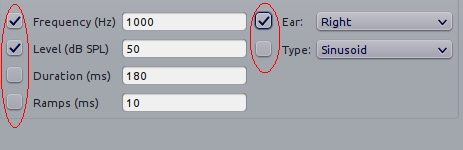
\includegraphics{Figures/inSummaryCheckBoxes.png}
   \label{fig:inSummaryCheckBoxes}
 \end{figure}
 In the example shown in Figure~\ref{fig:inSummaryCheckBoxes} the frequency, level and ear 
parameters will be stored, each in a separate column, in the block summary table (``\_table'') 
file, while the parameters corresponding to the unchecked boxes (duration, ramps and type) will be not. 
This is useful if you are running an experiment in which you are systematically 
varying only a few parameters across different blocks, and want to keep track of 
only those parameters. The \texttt{inSummary} check boxes also provide visual 
landmarks for quickly spotting the widgets with your parameters of interest in \texttt{pychoacoustics}.

Notice that the ``Process Results Table'' function, as mentioned in the previous 
section, will average the results for blocks with the same parameters 
stored in the block summary table (``\_table'') file.
This means that if you are varying a certain parameter (e.g., level) 
across blocks, but you don't check the corresponding \texttt{inSummary} check box (for each block), the value
of the parameter will not be stored in the block summary table (``\_table'') file, 
and as a consequence the ``Process Results Table'' function will not be able 
to sort the blocks according to the ``level'' parameter, and will average the 
results across all blocks. Not all is lost, because the ``level'' parameter will be nonetheless stored in the
``block summary'' file, but you will need more work before you can process your results with a statistical software package.

\subsubsection{Log Results Files}
\texttt{pychoacoustics} automatically saves backup copies of the ``block summary'' and ``full'' files in a backup folder. 
On Linux systems this folder is located in 
\begin{verbatim}
~/.local/share/data/pychoacoustics/data_backup
\end{verbatim}
on Windows systems it is located in
\begin{verbatim}
C:\\Users\username\.local\share\data\pychoacoustics\data_backup
\end{verbatim}
where \texttt{username} is your account login name.
A separate file is saved for each block of trials that is run. These files are named according to
the date and time at which the blocks were started (the naming follows the YY-MM-DD-HH-MM-SS scheme). 
Unlike other results files, that are written only once a block of trials has been completed,
these log results files get written as soon as information is available (e.g., a new line
in the ``full'' results file is written at the end of each trial).

\subsubsection{Adaptive and Weighted Up/Down Result Files}
\subsubsection{Adaptive and Weighted Up/Down Interleaved Result Files}
\subsection{Constant m-Intervals n-Alternatives Result Files}
\subsection{Multiple Constants m-Intervals n-Alternatives Result Files}
\subsection{Constant 1-Intervals 2-Alternatives Result Files}
\subsection{Multiple Constants 1-Intervals 2-Alternatives Result Files}
\subsection{Constant 1-Pair Same/Different Result Files}
\section{Block Presentation Position}
\label{sec:shuffling}

%The presentation of the blocks during an experimental session can be randomized,
%while the order in which the blocks are stored in a parameters file remains invariant. 
We will define the serial position at which a block is presented
during an experimental session as its ``presentation position'', and the serial
position at which a block is stored in a parameters file as its ``storage point''.

Clicking the ``Shuffle'' button randomises the presentation positions of the blocks, but leaves
the order in which the blocks are stored in a parameters file untouched. The ``Previous'' and ``Next'' buttons,
as well as the ``Jump to Block'' chooser let you navigate across the blocks storage points, while the 
``Previous Position'', and the ``Next Position'' buttons,
as well as the ``Jump to Position'' chooser let you navigate across the blocks presentation
positions. 

The block presentation positions are recorded in the parameters files. This is useful in case you have 
to interrupt an experimental session whose block presentation positions had been randomized, before it is finished, and continue it at a later date.
In this case you can save the parameters file, reload it next time, and let the listener complete the experimental blocks
that s/he had not run because of the interruption. Notice that each time you load a parameters file \texttt{pychoacoustics} will automatically
move to the first block presentation position. Therefore, you will have to note down what was the last block that your listener had run in the interrupted 
session (or find out by looking at the results file) and move to the presentation position of the following block yourself.

By default clicking on the ``Shuffle'' button performs a simple full randomization of the block presentation positions.
However, you can specify more complex shuffling schemes in the ``Shuffling Scheme'' text field. Let's say you want to
present two tasks in your experiment, a frequency discrimination and an intensity discrimination task. Each task
has four subconditions, (e.g.\ four different base frequencies for the frequency discrimination task and four
different base intensities for the intensity discrimination task). Your parameters file will contain eight blocks in total,
blocks one to four are for the frequency discrimination task and blocks five to eight are for the intensity discrimination task.
During the experiment you want your participants to run first the four frequency discrimination conditions in random order, and afterwards the
four intensity discrimination conditions in random order. To achieve this you can enter the following shuffling scheme:
\begin{verbatim}
([1,2,3,4], [5,6,7,8])
\end{verbatim}
basically you specify sequences (which can be nested) with your experimental blocks, sequences within round parentheses \texttt{()} are
not shuffled, while sequences within square brackets \texttt{[]} are shuffled. Following the previous example, if you want to present
first the four blocks of one of the tasks (either frequency or intensity) in random order, and then the four blocks of the other task
in random order, you would specify your shuffling scheme as follows:
\begin{verbatim}
[[1,2,3,4], [5,6,7,8]]
\end{verbatim}
on the other hand, if you want to present first the four blocks of one of the tasks (either frequency or intensity)
in sequential order and then the four blocks of the other task in sequential order, you would specify your shuffling scheme
as follows:
\begin{verbatim}
[(1,2,3,4), (5,6,7,8)]
\end{verbatim}
you can have any variation you like on the theme, and the lists can be nested ad libitum, so for example
you could have:
\begin{verbatim}
[(1,2,[3,4]), (5,6,7,8)]
\end{verbatim}
this would instruct \texttt{pychoacoustics} to present first either the four frequency conditions
or the four intensity conditions. The first two frequency conditions are presented sequentially,
while the last two are shuffled. To save typing you can give ranges rather than listing all blocks individually.
For example:
\begin{verbatim}
([1-4], [5-8])
\end{verbatim}
is equivalent to:
\begin{verbatim}
([1,2,3,4], [5,6,7,8])
\end{verbatim}






\section{OS Commands}
\label{sec:end_cmd}

\texttt{pychoacoustics} can be instructed to run operating system (OS) commands
at the end of an experiment. This may be useful to run custom scripts that may
analyse the result files, backup result files or perform other operations. 

In the control window, you can enter commands that you want to be executed at the
end of a specific experiment in the "End Command" box. This command will be saved
in the parameters file of the experiment.

In the "Preferences Dialog", under the "Notifications" tab you can instead set a command
that will be executed at the end of each experiment you run, or $n$ blocks before the end of each experiment you run. 
These commands should be entered in the "Execute custom command" boxes.

The commands that you can execute are OS commands, therefore they are different on Linux
and Windows platforms. On Linux, for example, assuming that you store all your experimental
results in the directory "/home/foo/exp/", you could automatically make a backup of these
files in the directory "/home/foo/backup/exp/" by using the command
\begin{verbatim}
rsync -r -t -v --progress -s /home/foo/exp/ /home/foo/backup/exp/
\end{verbatim}

To make things more interesting, you can use some special strings to pass \texttt{pychoacoustics}
internal variables to your commands. For example, if you want to copy the results file of
the current experiment to the directory "/home/foo/res/", you can use the command
\begin{verbatim}
cp [resFile] /home/foo/backup/exp/
\end{verbatim}
here the special string \verb+[resFile]+ will be converted to the name of the file where \texttt{pychoacoustics}
has saved the data. A full listing of these special strings is given in Table~\ref{tab:end_cmd}.

\begin{table}[htbp]
\caption{Special strings for OS end command.} 
\begin{tabular}{ll}
\toprule

\textbf{String} & \textbf{Variable}  \\
%"[resDir]", "[resFile]",        "[resFileFull]", "[resFileRes]", "[resTable]", "[listener]", "[experimenter]"
\midrule
\verb+[resDir]+ & Results file directory \\
\verb+[resFile]+ & Block summary results file \\
\verb+[resFileFull]+ & Full results file \\
\verb+[resFileRes]+ & Session summary results file \\
\verb+[resTable]+ & Block summary table results file \\
\verb+[listener]+  & Listener label \\
\verb+[experimenter]+  & Experimenter ID \\

\bottomrule
\end{tabular}
\label{tab:end_cmd}
\end{table}

\section{Preferences Settings}
\label{sec:preferences}
All the settings that can be manipulated in the ``Preferences'' dialog, as 
well as the ``Phones'' and ``Experimenters'' dialogs are stored in a file 
in the user home directory. On Linux this file is located in:
\begin{verbatim}
~/.config/pychoacoustics/preferences.py
\end{verbatim}
On Windows, assuming the root drive is ``C'' it is located in:
\begin{verbatim}
C:\\Users\username\.config/pychoacoustics\preferences.py
\end{verbatim}
where \verb+username+ is your Windows login username.
Although I strive to avoid this, the way in which the preferences settings are stored 
may change in newer versions of pychoacoustics. This means that when pychoacoustics is 
upgraded to a newer version it may sometimes not start or throw out errors. To address 
these issues, please, try removing the old preferences file. Of course this means that 
you're going to lose all the settings that you had previously saved. To avoid loosing 
any precious information, such as the calibration values of your headphones, write down 
all important info before removing the preferences file.


\section{Response Mode}
\label{sec:response_mode}

\texttt{pychoacoustics} was designed to run interactive experiments in which a listener
hears some stimuli and gives a response through a button or key press. This is the default
mode, called ``Real Listener'' mode. \texttt{pychoacoustics} provides two additional response
modes, ``Automatic'' and ``Simulated Listener''. These modes can be set through the control window.

In ``Automatic'' response mode, rather than waiting for the listener to give a response,
\texttt{pychoacoustics} gives itself a response and proceeds to the next trial. The probability
that this automatic response is correct can also be set through the control window.
The ``Automatic'' response mode has two main functions. The first is testing and debugging
an experiment. Rather than running the experiment yourself, you can launch \texttt{pychoacoustics}
in ``Automatic'' response mode and check that everything runs smoothly, the program doesn't crash,
and the result files are saved correctly. The second function of the automatic response mode is to allow
passive presentation of the stimuli. Some neuroimaging experiments (e.g.\ electroencephalographic or
functional magnetic resonance recordings) are performed with listeners passively listening to the stimuli.
These experiments usually also require that the program presenting the stimuli sends triggers to the
recording equipment to flag the start of a trial. Potentially this can also be done in \texttt{pychoacoustics}
(and we've done it in our lab for electroencephalographic recordings), but at the moment this functionality
is not implemented in a general way in the program.

The ``Simulated Listener'' mode is simply a hook that allows you to redirect the control flow of the program 
to some code that simulates a listener and provides a response. Notice that \texttt{pychoacoustics} does not
provide any simulation code in itself, the simulation code has to be written by you for a specific experiment.
If no simulation code is written in the experiment file, \texttt{pychoacoustics} will do nothing in simulated
listenr mode. Further details on how to use the ``Simulated Listener'' mode are provided in Section~\ref{sec:simulations}.

Both the ``Automatic'' and the ``Simulated Listener'' make recursive function calls. In Python the number of recursive function
calls that you can make is limited. If your experiment passes this limit \texttt{pychoacoustics} will crash. The limit can be
raised, up to a certain extent (which is dependent on your operating system, see the documentation for the setrecursionlimit function in the Python \texttt{sys} module) through the ``Max Recursion Depth'' setting that you can
find in the preferences window, or set through a command line option when running \texttt{pychoacoustics} from the command line.
Notice that the total number of recursive calls that your program will make to complete an experiments will be higher than the number of
trials in the experiment, so you should set the ``Max Recursion Depth'' to a value higher than the number of trials you're planning
to perform (how much higher I don't know, you should find out by trial and error, a few hundred points higher is usually sufficient).
If you're planning to run a very high number of trials in ``Automatic'' or ``Simulated Listener'' mode, rather than raising 
the max recursion depth, it may be better to split the experiment in several parts. You can always write a script that automatically
launches \texttt{pychoacoustics} from the command line instructing it to load a given parameters file. On UNIX machines you could write a shell script to do that, 
but an easier way is perhaphs to use python itself to write the script. For example, the \texttt{python} script could be:
\begin{lstlisting}
#! /usr/bin/env python
for i in range(5):
   cmd = "pychoacoustics --file prms.prm -l L1 -s s1 -q -a \
         --recursion-depth 3000" 
\end{lstlisting}[
here we're telling \texttt{pychoacoustics} to load the parameters file \texttt{prms.prm}, set the listener identifier to ``L1'' and the session label to s1. 
The \texttt{-q} option instructs the program to exit at the end of the experiment. 
This way the recursion depth count is effectively restarted each time \texttt{pychoacoustics} is closed and launched again from the script. 
When the \verb+--recursion-depth+ option is passed as a command line argument, as in the example above, it overrides 
the max recursion depth value set in the preferences window. If the \verb+-a+ option is passed, as in the examples above, \texttt{pychoacoustics} will start
automatically at the beginning of each of the five series . This is useful for debugging or simulations, so that you can start the script and
leave the program complete unattended (you need to make sure that the ``Shuffling Mode'' is not set to ``Ask'' and that you pass listener
and session labels if you want the program to run completely unattended). 

%%% Local Variables: 
%%% mode: latex
%%% TeX-master: "pychoacoustics_manual"
%%% End: 


\chapter{Designing Custom Experiments}
\label{sec:cutom_exp}

In order to add a new experiment to \texttt{pychoacoustics}, create a directory in your home folder called \texttt{pychoacoustics\_experiments}, inside this folder create a subfolder called \texttt{custom\_experiments}. Each experiment is written in a single file contained in this folder. Let's imagine we want to create an experiment for a simple frequency discrimination task. We create a file named \verb+freq.py+ in the \texttt{custom\_experiments} folder. In addition to the experiment file we need an additional file that lists all the experiments contained in the \texttt{custom\_experiments} directory. This file must be named \verb+__init__.py+, and in our case it will have the following content:
\begin{lstlisting}[stepnumber=0]
__all__ = ["freq"]
\end{lstlisting}


here the variable \verb+__all__+ is simply a python list with the name of the experiment files. So, if one day we decide to write a new experiment on, let's say, level discrimination, in a file called \verb+lev.py+ we would simply add it to the list in \verb+__init__.py+:
\begin{lstlisting}[stepnumber=0]
__all__ = ["freq",
           "lev"]
\end{lstlisting}
For people familiar with packaging Python modules it should be clear by now that the custom experiments folder is basically a Python package containing various modules (the experiment files). If at some point we want to remove an experiment from \texttt{pychoacoustics}, for example because it contains a bug that does not allow the program to start, we can simply remove it from the list in \verb+__init__.py+

Let's go back to the \verb+freq.py+ file. Here we need to define four functions. For our example the names of these functions would be:
\begin{lstlisting}[stepnumber=0]
initialize_freq()
select_default_parameters_freq()
get_fields_to_hide_freq()
doTrial_freq()
\end{lstlisting}
basically the function names consist of a fixed prefix, followed by the name of the experiment file. So in the case of the level experiment example written in the file \verb+lev.py+, our four functions would be called:
\begin{lstlisting}[stepnumber=0]
initialize_lev()
select_default_parameters_lev()
get_fields_to_hide_lev()
doTrial_lev()
\end{lstlisting}
we'll look at each function in details shortly. Briefly, the \verb+initialize_+ function is used to set some general parameters and options for our experiment; the \verb+select_default_parameters_+ function lists all the widgets (text fields and choosers) of our experiment and their default values; the \verb+get_field_to_hide_+ function is used to dinamically hide or show certain widgets depending on the status of other widgets; finally, the \verb+doTrial_+ function contains the code that generates the sounds and plays them during the experiment.

\subsubsection{The \texttt{initialize\_} function}
The \verb+initialize_+ function of our frequency discrimination experiment looks like this:
\begin{lstlisting}
def initialize_freq(prm):
  exp_name = "Frequency Discrimination Demo"
  prm["experimentsChoices"].append(exp_name)
  prm[exp_name] = {}
  prm[exp_name]["paradigmChoices"] = ["Adaptive",
                                      "Weighted Up/Down",
                                      "Constant m-Intervals n-Alternatives"]

  prm[exp_name]["opts"] = ["hasISIBox", "hasAlternativesChooser", 
                           "hasFeedback", "hasIntervalLights"]
    
  prm[exp_name]["execString"] = "freq"
  return prm
\end{lstlisting}
When the function is called, it is passed a dictionary containing various parameters through the ``prm'' argument.
The function receives this dictionary of parameters and adds or modifies some of them.
In the first line we give a label to the experiment, this can be anything we want, except the label of an experiment already existing.
The second line adds this experiment label to the list of ``experimentsChoices''.
The third line creates a new sub-dictionary that has as a key the experiment label.
Next we list the paradims that our experiment supports by creating a ``paradigmChoices'' key and giving
the names of the supported paradigms as a list. These paradims listed here must be within the set of paradims 
supported by \texttt{pychoacoustics} (see Section~\ref{sec:paradigms} for a description of the paradigms currently supported).
In the next line we set an ``\texttt{opts}'' key containing a list of options. The full list of options that can be set here
is described in details in Section~\ref{sec:experiment_opts}. In brief, for our experiment we want to have a widget to set the ISI between presentation
intervals (\texttt{hasISIBox}), a widget to choose the number of response alternatives (\texttt{hasAlternativesChooser}),
a widget to set the feedback on or off for a given block of trials (\texttt{hasFeedback}), and finally we want lights
to mark the observation intervals (\texttt{hasIntervalLights}).
The penultimate line of the \verb+initialize_+ function sets the ``\texttt{execString}'' of our experiment. This
must be the name of our experiment file, so in our case ``\texttt{freq}''.



\subsubsection{The \texttt{select\_default\_parameters\_} function}
The \texttt{select\_default\_parameters\_} function is the function in which you
define all the widgets (text fields and choosers) needed for your experiment.
For our frequency discrimination experiment, the first lines look as follow:
\begin{lstlisting}
def select_default_parameters_freq(parent, paradigm, par):
   
  field = []
  fieldLabel = []
  chooser = []
  chooserLabel = []
  chooserOptions = []
\end{lstlisting}
the function accepts three arguments, ``parent'' is simply a reference to the pychoacoustics
application. ``paradigm'' is the paradigm with which the
function has been called, while ``par'' is a variable
that can hold some special values for initializing the function. The use of the ``par'' argument is discussed in Section~\ref{sec:par}.

From line three to line seven, we create a series of empty lists. The \texttt{field} and \texttt{fieldLabel } lists will
hold the default values of our text field widgets, and their labels, respectively. The \texttt{chooser} and \texttt{chooserLabel}
lists will likewise hold the default values of our chooser widgets, and their labels, while the \texttt{chooserOptions} list will hold 
the possible values that our choosers can take. Lines 8 to 29 show how we populate these lists for our frequency discrimination
experiment:

\begin{lstlisting}[firstnumber=8]
  fieldLabel.append("Frequency (Hz)")
  field.append(1000)

  fieldLabel.append("Starting Difference (%)")
  field.append(20)
    
  fieldLabel.append("Level (dB SPL)")
  field.append(50)
   
  fieldLabel.append("Duration (ms)")
  field.append(180)
    
  fieldLabel.append("Ramps (ms)")
  field.append(10)

    
  chooserOptions.append(["Right",
                         "Left",
                         "Both"])
  chooserLabel.append("Ear:")
  chooser.append("Right")
\end{lstlisting}

The last lines of our \texttt{select\_default\_parameters\_} function are used to set some additional parameters and look as follows:
\begin{lstlisting}[firstnumber=29]
  prm = {}
  if paradigm == None:
      prm['paradigm'] = "Adaptive"
  else:
      prm['paradigm'] = paradigm
  prm['adType'] =  "Geometric"
  prm['field'] = field
  prm['fieldLabel'] = fieldLabel
  prm['chooser'] = chooser
  prm['chooserLabel'] = chooserLabel
  prm['chooserOptions'] =  chooserOptions
  prm['nIntervals'] = 2
  prm['nAlternatives'] = 2

  return prm
\end{lstlisting}
on line 29 we create a dictionary to hold the parameters. Lines 30--33 are used to
set a default paradigm for our experiment if \texttt{None} has been passed to our function.
\texttt{'adType} gives sets the default type of the adaptive procedure, this could be either \texttt{Geometric}, or 
\texttt{Arithmetic}. From line 25 to line 39 we insert in the dictionary the \texttt{field}, \texttt{fieldLabel},
\texttt{chooser}, \texttt{chooserLabel} and \texttt{chooserOptions} lists that we have previously creaetd and populated.
Finally in the last two lines we give the default number of response intervals and response alternatives.

\subsubsection{The \texttt{get\_fields\_to\_hide\_} function}

The purpose of the \verb+get_fields_to_hide_+ function is to dinamically show or
hide certain widgets depending on the status of other widgets. This function must
be defined, but is not essential to a \texttt{pychoacoustics} experiment, so if you want to read
all the essential information first, you can simply write the following:
\begin{lstlisting}
def get_fields_to_hide_freq(parent):
  pass
\end{lstlisting}
and move on to read about the next function, otherwise, read on.

Let's suppose that you 
want to set up a frequency discrimination experiment in which the frequency of the 
standard stimulus may be either fixed, or change from trial to trial. You start by writing
an experiment with a single ``Frequency'' text field for the fixed stimulus frequency case.
You then add two additional fields called ``Min. Frequency'' and ``Max Frequency'' to set
the range of frequencies in the roving frequency case. Finally, you create a chooser to decide
whether an experiment is to be run with a fixed or roving frequency. The code for creating these widgets
is shown below:



\subsubsection{The \texttt{doTrial\_} function}

\subsubsection{The Experiment ``opts''}
\label{sec:experiment_opts}

\begin{itemize}
\item \verb+hasISIBox+
\item \verb+hasAlternativesChooser+
\item \verb+hasFeedback+
\item \verb+hasIntervalLights+
\item \verb+hasPreTrialInterval+
\end{itemize}

\subsubsection{Using \texttt{par}}
\label{sec:par}



\section{Simulations}
\label{sec:simulations}

\texttt{pychoacoustics} is not designed to run simulations in itself, however it provides a hook
to redirect the control flow to an auditory model that you need to specify yourself in the experiment file.

You can retrieve the current response mode from the experiment file with:
\begin{lstlisting}[stepnumber=0]
parent.prm['allBlocks']['responseMode']
\end{lstlisting}
so, in the experiment file, after the creation of the stimuli for the trial you can redirect the
control flow of the program depending on the response mode:
\begin{lstlisting}
if parent.prm['allBlocks']['responseMode'] != "Simulated Listener":
   #we are not in simulation mode, play the stimuli for the listener
   parent.playSoundSequence(sndSeq, ISIs)
if parent.prm['allBlocks']['responseMode'] == "Simulated Listener":
   #we are in simulation mode
   #pass the stimuli to an auditory model and decision device
   #---
   #Here you specify your model, pychoacoustics doesn't do it for you!
   # at the end your simulated listener arrives to a response that is
   # either correct or incorrect
   #---
   parent.prm['trialRunning'] = False 
   #this is needed for technical reasons (if the 'trialRunning'
   #flag were set to 'True' pychoacoustics would not process
   #the response.
   #
   #let's suppose that at the end of the simulation you store the
   #response in a variable called 'resp', that can take as values 
   #either the string 'Correct' or the string 'Incorrect'.
   #You can then proceed to let pychoacoustics process the response:
   #
   if resp == 'Correct':
      parent.sortResponse(parent.correctButton) 
   elif resp == 'Incorrect':
      #list all the possible 'incorrect' buttons
      inc_buttons = numpy.delete(numpy.arange(
                                 self.prm['nAlternatives'])+1, 
                                 self.correctButton-1))
      #choose one of the incorrect buttons
      parent.sortResponse(random.choice(inc_buttons))

\end{lstlisting}
%%% Local Variables: 
%%% mode: latex
%%% TeX-master: "pychoacoustics_manual"
%%% End: 


\chapter{Troubleshooting}

\subsubsection{The computer crashed in the middle of an experimental session}
\texttt{pychoacoustics} saves the results at the end of each block, therefore  only the results from the last uncompleted block will be lost, the results of completed blocks will not be lost. If you have an experiment with many different blocks presented in random order it may be difficult to see which blocks the listener had already completed and set \texttt{pychoacoustics} to run only the blocks that were not run. To address this issue \texttt{pychoacoustics} keeps a copy of the parameters, including the block presentation order after shuffling, in a file called \texttt{.tmp\_prm.prm} (this is a hidden file on Linux systems). Therefore, after the crash you can simply load this parameters file and move to the block position that the listener was running when the computer crashed to resume the experiment. 

A second function of the \texttt{.tmp\_prm.prm} file is to keep a copy of parameters that were stored in memory, but not saved to a file. If your computer crashed while you were setting up a parameters for an experiment that were not yet saved (or were only partially saved) to a file, you can retrieve them after the crash by loading the \texttt{.tmp\_prm.prm} file. One important thing to keep in mind is that the \texttt{.tmp\_prm.prm} will be overwritten as soon as new parameters are stored in memory by a \texttt{pychoacoustics} instance opened in the same directory. Therefore it is advisable to make a copy of the \texttt{.tmp\_prm.prm} file renaming it to avoid accidentally loosing its contents after the crash.



%%% Local Variables: 
%%% mode: latex
%%% TeX-master: "pychoacoustics_manual"
%%% End: 

\bibliographystyle{apacite}
\bibliography{biblio}

\appendix
\chapter{Introduction to Python, Numpy and Scipy}




%%% Local Variables: 
%%% mode: latex
%%% TeX-master: "pychoacoustics_manual"
%%% End: 


%---------The file header---------------------------------------------
%\documentclass[a4paper,12pt]{book} % possibilities : report book article , etc.

%\usepackage[english]{babel} %language selection
%\usepackage[T1]{fontenc}

%\pagenumbering{arabic}

%\usepackage{hyperref}
%\hypersetup{colorlinks, 
%           citecolor=black,
%           filecolor=black,
%           linkcolor=black,
%           urlcolor=black,
%           pdftex}

           
%\begin{document}
%---------------------------------------------------------------------
\chapter{GNU Free Documentation License}
%\label{label_fdl}

 \begin{center}

       Version 1.2, November 2002


 Copyright \copyright 2000,2001,2002  Free Software Foundation, Inc.
 
 \bigskip
 
     51 Franklin St, Fifth Floor, Boston, MA  02110-1301  USA
  
 \bigskip
 
 Everyone is permitted to copy and distribute verbatim copies
 of this license document, but changing it is not allowed.
\end{center}


\begin{center}
{\bf\large Preamble}
\end{center}

The purpose of this License is to make a manual, textbook, or other
functional and useful document "free" in the sense of freedom: to
assure everyone the effective freedom to copy and redistribute it,
with or without modifying it, either commercially or noncommercially.
Secondarily, this License preserves for the author and publisher a way
to get credit for their work, while not being considered responsible
for modifications made by others.

This License is a kind of "copyleft", which means that derivative
works of the document must themselves be free in the same sense.  It
complements the GNU General Public License, which is a copyleft
license designed for free software.

We have designed this License in order to use it for manuals for free
software, because free software needs free documentation: a free
program should come with manuals providing the same freedoms that the
software does.  But this License is not limited to software manuals;
it can be used for any textual work, regardless of subject matter or
whether it is published as a printed book.  We recommend this License
principally for works whose purpose is instruction or reference.


\begin{center}
{\Large\bf 1. APPLICABILITY AND DEFINITIONS}
\addcontentsline{toc}{section}{1. APPLICABILITY AND DEFINITIONS}
\end{center}

This License applies to any manual or other work, in any medium, that
contains a notice placed by the copyright holder saying it can be
distributed under the terms of this License.  Such a notice grants a
world-wide, royalty-free license, unlimited in duration, to use that
work under the conditions stated herein.  The \textbf{"Document"}, below,
refers to any such manual or work.  Any member of the public is a
licensee, and is addressed as \textbf{"you"}.  You accept the license if you
copy, modify or distribute the work in a way requiring permission
under copyright law.

A \textbf{"Modified Version"} of the Document means any work containing the
Document or a portion of it, either copied verbatim, or with
modifications and/or translated into another language.

A \textbf{"Secondary Section"} is a named appendix or a front-matter section of
the Document that deals exclusively with the relationship of the
publishers or authors of the Document to the Document's overall subject
(or to related matters) and contains nothing that could fall directly
within that overall subject.  (Thus, if the Document is in part a
textbook of mathematics, a Secondary Section may not explain any
mathematics.)  The relationship could be a matter of historical
connection with the subject or with related matters, or of legal,
commercial, philosophical, ethical or political position regarding
them.

The \textbf{"Invariant Sections"} are certain Secondary Sections whose titles
are designated, as being those of Invariant Sections, in the notice
that says that the Document is released under this License.  If a
section does not fit the above definition of Secondary then it is not
allowed to be designated as Invariant.  The Document may contain zero
Invariant Sections.  If the Document does not identify any Invariant
Sections then there are none.

The \textbf{"Cover Texts"} are certain short passages of text that are listed,
as Front-Cover Texts or Back-Cover Texts, in the notice that says that
the Document is released under this License.  A Front-Cover Text may
be at most 5 words, and a Back-Cover Text may be at most 25 words.

A \textbf{"Transparent"} copy of the Document means a machine-readable copy,
represented in a format whose specification is available to the
general public, that is suitable for revising the document
straightforwardly with generic text editors or (for images composed of
pixels) generic paint programs or (for drawings) some widely available
drawing editor, and that is suitable for input to text formatters or
for automatic translation to a variety of formats suitable for input
to text formatters.  A copy made in an otherwise Transparent file
format whose markup, or absence of markup, has been arranged to thwart
or discourage subsequent modification by readers is not Transparent.
An image format is not Transparent if used for any substantial amount
of text.  A copy that is not "Transparent" is called \textbf{"Opaque"}.

Examples of suitable formats for Transparent copies include plain
ASCII without markup, Texinfo input format, LaTeX input format, SGML
or XML using a publicly available DTD, and standard-conforming simple
HTML, PostScript or PDF designed for human modification.  Examples of
transparent image formats include PNG, XCF and JPG.  Opaque formats
include proprietary formats that can be read and edited only by
proprietary word processors, SGML or XML for which the DTD and/or
processing tools are not generally available, and the
machine-generated HTML, PostScript or PDF produced by some word
processors for output purposes only.

The \textbf{"Title Page"} means, for a printed book, the title page itself,
plus such following pages as are needed to hold, legibly, the material
this License requires to appear in the title page.  For works in
formats which do not have any title page as such, "Title Page" means
the text near the most prominent appearance of the work's title,
preceding the beginning of the body of the text.

A section \textbf{"Entitled XYZ"} means a named subunit of the Document whose
title either is precisely XYZ or contains XYZ in parentheses following
text that translates XYZ in another language.  (Here XYZ stands for a
specific section name mentioned below, such as \textbf{"Acknowledgements"},
\textbf{"Dedications"}, \textbf{"Endorsements"}, or \textbf{"History"}.)  
To \textbf{"Preserve the Title"}
of such a section when you modify the Document means that it remains a
section "Entitled XYZ" according to this definition.

The Document may include Warranty Disclaimers next to the notice which
states that this License applies to the Document.  These Warranty
Disclaimers are considered to be included by reference in this
License, but only as regards disclaiming warranties: any other
implication that these Warranty Disclaimers may have is void and has
no effect on the meaning of this License.


\begin{center}
{\Large\bf 2. VERBATIM COPYING}
\addcontentsline{toc}{section}{2. VERBATIM COPYING}
\end{center}

You may copy and distribute the Document in any medium, either
commercially or noncommercially, provided that this License, the
copyright notices, and the license notice saying this License applies
to the Document are reproduced in all copies, and that you add no other
conditions whatsoever to those of this License.  You may not use
technical measures to obstruct or control the reading or further
copying of the copies you make or distribute.  However, you may accept
compensation in exchange for copies.  If you distribute a large enough
number of copies you must also follow the conditions in section 3.

You may also lend copies, under the same conditions stated above, and
you may publicly display copies.


\begin{center}
{\Large\bf 3. COPYING IN QUANTITY}
\addcontentsline{toc}{section}{3. COPYING IN QUANTITY}
\end{center}


If you publish printed copies (or copies in media that commonly have
printed covers) of the Document, numbering more than 100, and the
Document's license notice requires Cover Texts, you must enclose the
copies in covers that carry, clearly and legibly, all these Cover
Texts: Front-Cover Texts on the front cover, and Back-Cover Texts on
the back cover.  Both covers must also clearly and legibly identify
you as the publisher of these copies.  The front cover must present
the full title with all words of the title equally prominent and
visible.  You may add other material on the covers in addition.
Copying with changes limited to the covers, as long as they preserve
the title of the Document and satisfy these conditions, can be treated
as verbatim copying in other respects.

If the required texts for either cover are too voluminous to fit
legibly, you should put the first ones listed (as many as fit
reasonably) on the actual cover, and continue the rest onto adjacent
pages.

If you publish or distribute Opaque copies of the Document numbering
more than 100, you must either include a machine-readable Transparent
copy along with each Opaque copy, or state in or with each Opaque copy
a computer-network location from which the general network-using
public has access to download using public-standard network protocols
a complete Transparent copy of the Document, free of added material.
If you use the latter option, you must take reasonably prudent steps,
when you begin distribution of Opaque copies in quantity, to ensure
that this Transparent copy will remain thus accessible at the stated
location until at least one year after the last time you distribute an
Opaque copy (directly or through your agents or retailers) of that
edition to the public.

It is requested, but not required, that you contact the authors of the
Document well before redistributing any large number of copies, to give
them a chance to provide you with an updated version of the Document.


\begin{center}
{\Large\bf 4. MODIFICATIONS}
\addcontentsline{toc}{section}{4. MODIFICATIONS}
\end{center}

You may copy and distribute a Modified Version of the Document under
the conditions of sections 2 and 3 above, provided that you release
the Modified Version under precisely this License, with the Modified
Version filling the role of the Document, thus licensing distribution
and modification of the Modified Version to whoever possesses a copy
of it.  In addition, you must do these things in the Modified Version:

\begin{itemize}
\item[A.] 
   Use in the Title Page (and on the covers, if any) a title distinct
   from that of the Document, and from those of previous versions
   (which should, if there were any, be listed in the History section
   of the Document).  You may use the same title as a previous version
   if the original publisher of that version gives permission.
   
\item[B.]
   List on the Title Page, as authors, one or more persons or entities
   responsible for authorship of the modifications in the Modified
   Version, together with at least five of the principal authors of the
   Document (all of its principal authors, if it has fewer than five),
   unless they release you from this requirement.
   
\item[C.]
   State on the Title page the name of the publisher of the
   Modified Version, as the publisher.
   
\item[D.]
   Preserve all the copyright notices of the Document.
   
\item[E.]
   Add an appropriate copyright notice for your modifications
   adjacent to the other copyright notices.
   
\item[F.]
   Include, immediately after the copyright notices, a license notice
   giving the public permission to use the Modified Version under the
   terms of this License, in the form shown in the Addendum below.
   
\item[G.]
   Preserve in that license notice the full lists of Invariant Sections
   and required Cover Texts given in the Document's license notice.
   
\item[H.]
   Include an unaltered copy of this License.
   
\item[I.]
   Preserve the section Entitled "History", Preserve its Title, and add
   to it an item stating at least the title, year, new authors, and
   publisher of the Modified Version as given on the Title Page.  If
   there is no section Entitled "History" in the Document, create one
   stating the title, year, authors, and publisher of the Document as
   given on its Title Page, then add an item describing the Modified
   Version as stated in the previous sentence.
   
\item[J.]
   Preserve the network location, if any, given in the Document for
   public access to a Transparent copy of the Document, and likewise
   the network locations given in the Document for previous versions
   it was based on.  These may be placed in the "History" section.
   You may omit a network location for a work that was published at
   least four years before the Document itself, or if the original
   publisher of the version it refers to gives permission.
   
\item[K.]
   For any section Entitled "Acknowledgements" or "Dedications",
   Preserve the Title of the section, and preserve in the section all
   the substance and tone of each of the contributor acknowledgements
   and/or dedications given therein.
   
\item[L.]
   Preserve all the Invariant Sections of the Document,
   unaltered in their text and in their titles.  Section numbers
   or the equivalent are not considered part of the section titles.
   
\item[M.]
   Delete any section Entitled "Endorsements".  Such a section
   may not be included in the Modified Version.
   
\item[N.]
   Do not retitle any existing section to be Entitled "Endorsements"
   or to conflict in title with any Invariant Section.
   
\item[O.]
   Preserve any Warranty Disclaimers.
\end{itemize}

If the Modified Version includes new front-matter sections or
appendices that qualify as Secondary Sections and contain no material
copied from the Document, you may at your option designate some or all
of these sections as invariant.  To do this, add their titles to the
list of Invariant Sections in the Modified Version's license notice.
These titles must be distinct from any other section titles.

You may add a section Entitled "Endorsements", provided it contains
nothing but endorsements of your Modified Version by various
parties--for example, statements of peer review or that the text has
been approved by an organization as the authoritative definition of a
standard.

You may add a passage of up to five words as a Front-Cover Text, and a
passage of up to 25 words as a Back-Cover Text, to the end of the list
of Cover Texts in the Modified Version.  Only one passage of
Front-Cover Text and one of Back-Cover Text may be added by (or
through arrangements made by) any one entity.  If the Document already
includes a cover text for the same cover, previously added by you or
by arrangement made by the same entity you are acting on behalf of,
you may not add another; but you may replace the old one, on explicit
permission from the previous publisher that added the old one.

The author(s) and publisher(s) of the Document do not by this License
give permission to use their names for publicity for or to assert or
imply endorsement of any Modified Version.


\begin{center}
{\Large\bf 5. COMBINING DOCUMENTS}
\addcontentsline{toc}{section}{5. COMBINING DOCUMENTS}
\end{center}


You may combine the Document with other documents released under this
License, under the terms defined in section 4 above for modified
versions, provided that you include in the combination all of the
Invariant Sections of all of the original documents, unmodified, and
list them all as Invariant Sections of your combined work in its
license notice, and that you preserve all their Warranty Disclaimers.

The combined work need only contain one copy of this License, and
multiple identical Invariant Sections may be replaced with a single
copy.  If there are multiple Invariant Sections with the same name but
different contents, make the title of each such section unique by
adding at the end of it, in parentheses, the name of the original
author or publisher of that section if known, or else a unique number.
Make the same adjustment to the section titles in the list of
Invariant Sections in the license notice of the combined work.

In the combination, you must combine any sections Entitled "History"
in the various original documents, forming one section Entitled
"History"; likewise combine any sections Entitled "Acknowledgements",
and any sections Entitled "Dedications".  You must delete all sections
Entitled "Endorsements".

\begin{center}
{\Large\bf 6. COLLECTIONS OF DOCUMENTS}
\addcontentsline{toc}{section}{6. COLLECTIONS OF DOCUMENTS}
\end{center}

You may make a collection consisting of the Document and other documents
released under this License, and replace the individual copies of this
License in the various documents with a single copy that is included in
the collection, provided that you follow the rules of this License for
verbatim copying of each of the documents in all other respects.

You may extract a single document from such a collection, and distribute
it individually under this License, provided you insert a copy of this
License into the extracted document, and follow this License in all
other respects regarding verbatim copying of that document.


\begin{center}
{\Large\bf 7. AGGREGATION WITH INDEPENDENT WORKS}
\addcontentsline{toc}{section}{7. AGGREGATION WITH INDEPENDENT WORKS}
\end{center}


A compilation of the Document or its derivatives with other separate
and independent documents or works, in or on a volume of a storage or
distribution medium, is called an "aggregate" if the copyright
resulting from the compilation is not used to limit the legal rights
of the compilation's users beyond what the individual works permit.
When the Document is included in an aggregate, this License does not
apply to the other works in the aggregate which are not themselves
derivative works of the Document.

If the Cover Text requirement of section 3 is applicable to these
copies of the Document, then if the Document is less than one half of
the entire aggregate, the Document's Cover Texts may be placed on
covers that bracket the Document within the aggregate, or the
electronic equivalent of covers if the Document is in electronic form.
Otherwise they must appear on printed covers that bracket the whole
aggregate.


\begin{center}
{\Large\bf 8. TRANSLATION}
\addcontentsline{toc}{section}{8. TRANSLATION}
\end{center}


Translation is considered a kind of modification, so you may
distribute translations of the Document under the terms of section 4.
Replacing Invariant Sections with translations requires special
permission from their copyright holders, but you may include
translations of some or all Invariant Sections in addition to the
original versions of these Invariant Sections.  You may include a
translation of this License, and all the license notices in the
Document, and any Warranty Disclaimers, provided that you also include
the original English version of this License and the original versions
of those notices and disclaimers.  In case of a disagreement between
the translation and the original version of this License or a notice
or disclaimer, the original version will prevail.

If a section in the Document is Entitled "Acknowledgements",
"Dedications", or "History", the requirement (section 4) to Preserve
its Title (section 1) will typically require changing the actual
title.


\begin{center}
{\Large\bf 9. TERMINATION}
\addcontentsline{toc}{section}{9. TERMINATION}
\end{center}


You may not copy, modify, sublicense, or distribute the Document except
as expressly provided for under this License.  Any other attempt to
copy, modify, sublicense or distribute the Document is void, and will
automatically terminate your rights under this License.  However,
parties who have received copies, or rights, from you under this
License will not have their licenses terminated so long as such
parties remain in full compliance.


\begin{center}
{\Large\bf 10. FUTURE REVISIONS OF THIS LICENSE}
\addcontentsline{toc}{section}{10. FUTURE REVISIONS OF THIS LICENSE}
\end{center}


The Free Software Foundation may publish new, revised versions
of the GNU Free Documentation License from time to time.  Such new
versions will be similar in spirit to the present version, but may
differ in detail to address new problems or concerns.  See
http://www.gnu.org/copyleft/.

Each version of the License is given a distinguishing version number.
If the Document specifies that a particular numbered version of this
License "or any later version" applies to it, you have the option of
following the terms and conditions either of that specified version or
of any later version that has been published (not as a draft) by the
Free Software Foundation.  If the Document does not specify a version
number of this License, you may choose any version ever published (not
as a draft) by the Free Software Foundation.


\begin{center}
{\Large\bf ADDENDUM: How to use this License for your documents}
\addcontentsline{toc}{section}{ADDENDUM: How to use this License for your documents}
\end{center}

To use this License in a document you have written, include a copy of
the License in the document and put the following copyright and
license notices just after the title page:

\bigskip
\begin{quote}
    Copyright \copyright  YEAR  YOUR NAME.
    Permission is granted to copy, distribute and/or modify this document
    under the terms of the GNU Free Documentation License, Version 1.2
    or any later version published by the Free Software Foundation;
    with no Invariant Sections, no Front-Cover Texts, and no Back-Cover Texts.
    A copy of the license is included in the section entitled "GNU
    Free Documentation License".
\end{quote}
\bigskip
    
If you have Invariant Sections, Front-Cover Texts and Back-Cover Texts,
replace the "with...Texts." line with this:

\bigskip
\begin{quote}
    with the Invariant Sections being LIST THEIR TITLES, with the
    Front-Cover Texts being LIST, and with the Back-Cover Texts being LIST.
\end{quote}
\bigskip
    
If you have Invariant Sections without Cover Texts, or some other
combination of the three, merge those two alternatives to suit the
situation.

If your document contains nontrivial examples of program code, we
recommend releasing these examples in parallel under your choice of
free software license, such as the GNU General Public License,
to permit their use in free software.

%---------------------------------------------------------------------
%\end{document}


\end{document}